
\documentclass[cs, msthesis]{usuthesis}

\usepackage{epsfig}
\usepackage{amssymb}           % add ams symbols stuff
\usepackage{caption}		% needed for listing captions
\usepackage{graphicx}          	% add graphics
\usepackage{subfigure}
\usepackage{color}             	% grants control of link text colors.
\usepackage[usenames,dvipsnames,rgb]{xcolor}
\usepackage{algorithm2e}
\usepackage{listings}		% code listings
\usepackage{pdflscape}
\usepackage{hyperref}          	% make contents/ref/citations clickable
\usepackage{epstopdf}
\usepackage{enumerate}		% lists of items
\usepackage{url} 			% url in bib
\usepackage{tikz}
\usetikzlibrary{decorations.text}
\usepackage{tkz-berge}
\usepackage{mathtools}
\usepackage{tabu}
\usepackage{longtable}

% for formatting code
\lstset{
	language=C++,						% choose the language of the code
	basicstyle=\footnotesize,			% the size of the fonts that are used for the code
	numbers=left,						% where to put the line-numbers
	numberstyle=\footnotesize,			% the size of the fonts that are used for the line-numbers
	stepnumber=1,						% the step between two line-numbers. If it is 1 each line will be numbered
	firstnumber=0,
	lineskip={3pt},
	aboveskip={2\baselineskip},
	belowskip={0\baselineskip},
	xleftmargin=0mm,					% left margin of listing section
	floatplacement=t,
	numbersep=-15pt,					% how far the line-numbers are from the code
	backgroundcolor=\color{white},		% choose the background color. You must add \usepackage{color}
	showspaces=false,					% show spaces adding particular underscores
	showstringspaces=false,				% underline spaces within strings
	showtabs=false,						% show tabs within strings adding particular underscores
	frame=tb,							% adds a frame around the code
	tabsize=4,							% sets default tabsize to 2 spaces
	captionpos=b,						% sets the caption-position to bottom
	breaklines=true,					% sets automatic line breaking
	breakatwhitespace=false,			% sets if automatic breaks should only happen at whitespace
	numberbychapter=true,
	escapeinside={\%*}{*)}				% if you want to add a comment within your code
}
\lstloadlanguages{
	C++
 }

% https://tex.stackexchange.com/questions/42271/floor-and-ceiling-functions
\DeclarePairedDelimiter{\ceil}{\lceil}{\rceil}
\DeclarePairedDelimiter{\floor}{\lfloor}{\rfloor}

\intextsep=10mm							% controls spacing before and after figures and tables
\belowcaptionskip=-5mm

%Set all linked content to be plain black text
\hypersetup{
	colorlinks,
	citecolor=black,
	filecolor=black,
	linkcolor=black,
	urlcolor=black
}


% Author and Title Information
\author{Jesse Victors}
\title{EsgalDNS: \\ Tor-powered Distributed DNS \\ for Tor Hidden Services}


% The Committee
\majorprof{Dr. Ming Li}
\firstreader{Dr. Nicholas Flann}
\secondreader{Dr. Daniel Watson}


% Graduate Dean, Update as necessary
\graddean{Dr. Mark R. McLellan} 
\deantitle{Vice President for Research and}
\deansecondtitle{Dean of the School of Graduate Studies}

% Degree Information
\degree{Master of Science}
\month{May}
\year{2015}

\begin{document}

	%{{{ Frontmatter
	\preliminaries   % set frontmatter style

	\maketitle
	%\makecopyright        % optional
	
	%

\begin{abstract}
% A space is needed before the text starts so that the first paragraph
% is indented properly.

The Tor network is a second-generation onion routing system that aims to provide anonymity, privacy, and Internet censorship resistance to its users. In recent years it has grown significantly in response to revelations of national and global electronic surveillance, and remains one of the most popular and secure anonymity network in use today. Tor is also known for its support of anonymous websites within its network. Decentralized and secure, the domain names for these services are tied to public key infrastructure (PKI) but are challenged by their long and technical addresses. In response to this difficulty, in this thesis I introduce a novel and decentralized Tor-powered DNS system that provides unique and human-meaningful domain names to Tor hidden services.

\end{abstract}

	%\begin{publicabstract}
\centerline{Jesse M. Victors}
\vspace{12pt}

The Tor network is a third-generation onion router that aims to provide private and anonymous Internet access to its users. In recent years its userbase, network, and community has grown significantly in response to revelations of national and global electronic surveillance, and it remains one of the most popular anonymity networks in use today. Tor also provides access to anonymous servers known as hidden services -- servers of unknown location and ownership that may provide websites, chat services, or an electronic dead drop. These hidden services can be accessed through any Tor-powered web browser but they suffer from usability challenges due to the algorithmic generation and unmemorability of hidden service addresses. In response to this difficulty, in this work we introduce the Onion Name System (OnioNS), a distributed DNS that provides unique owner-selected domain names to Tor hidden services. OnioNS can be embedded in any fully-connected onion router, though here we describe its application inside the Tor network.

\end{publicabstract}

	
	%

\begin{dedication}
% A space is needed before the text starts so that the first paragraph
% is indented properly.

This work is dedicated to the developers and community behind the Tor Project and the Tails OS.

\end{dedication}
  % optional
	%
%https://tex.stackexchange.com/questions/656/how-to-create-acknowledgements-in-the-report-class
\begin{dedication}

The authors would like to thank Mark Ellzey, Yawning Angel, and Nick Mathewson for their assistance with libevent and Tor technical support; Sarbajit Mukherjee for his commentary; and the Tor community for their continued support.

\end{dedication}     % optional
	\tableofcontents
	%\listoftables
	\listoffigures

	%    \include{doc/notation}  % optional
	%    \include{doc/acronyms}  % optional
	%}}}
	%{{{ The main body of the thesis
	\body  % set main body style

	% Chapters
	
\chapter{INTRODUCTION}

\section{Onion Routing}

As the prevalence of the Internet and other communication has grown, so too has the development and usage of privacy-enhancing systems. These are tools and protocols that provide privacy by obfuscating the link between a user's identification or location and their communications. Privacy is not achieved in traditional Internet connections because SSL/TLS encryption cannot hide IP and TCP headers, which must be exposed to allow routing between two parties; eavesdroppers can easily break user privacy by monitoring these headers. A closely related property is anonymity -- a part of privacy where user activities cannot be tracked and their communications are indistinguishable from others. Tools that provide these systems hold a user's identity in confidence, and privacy and anonymity are often provided together. Following a general distrust of unsecured Internet communications and in light of the 2013-current revelations by Edward Snowden of Internet mass-surveillance by the NSA, GCHQ, and other members of the Five Eyes, users have increasingly turned to these tools for their own protection. Privacy-enhancing and anonymity tools may also be used by the military, researchers working in sensitive topics, journalists, law enforcement running tip lines, activists and whistleblowers, or individuals in countries with Internet censorship. These users may turn to proxies or VPNs, but these tools often track their users for liability reasons and thus rarely provide anonymity. Furthermore, they can easily voluntarily or be forced to break confidence to destroy user privacy. More complex tools are needed for a stronger guarantee of privacy and anonymity.

Today, most anonymity tools descend from mixnets, an early anonymity system invented by David Chaum in 1981.\cite{chaum2003untraceable} In a mixnet, user messages are transmitted to one or more mixes, who each partially decrypt, scramble, delay, and retransmit the messages to other mixes or to the final destination. This enhances privacy by heavily obscuring the correlation between the origin, destination, and contents of the messages. Mixnets have inspired the development of many varied mixnet-like protocols and have generated significant literature within the field of network security.\cite{edman2009anonymity}\cite{syverson2011peel}

Mixnet descendants can generally be classified into two distinct categories: high-latency and low-latency systems. High-latency networks typically delay traffic packets and are notable for their greater resistance to global adversaries who monitor communication entering and exiting the network. However, high-latency networks, due to their slow speed, are typically not suitable for common Internet activities such as web browsing, instant messaging, or the prompt transmission of email. Low-latency networks, by contrast, do not delay packets and are thus more suited for these activities, but they are more vulnerable to timing attacks from global adversaries.\cite{dingledine2004tor} In this work, we detail and introduce new functionality within low-latency protocols.

Onion routing is a technique for enhancing privacy of TCP-based communication across a network and is the most popular low-latency descendant of mixnets in use today. It was first designed by the U.S. Naval Research Laboratory in 1997 for military applications\cite{syverson1997anonymous}\cite{reed1998anonymous} but has since seen widespread usage. In onion routing with public key infrastructure (PKI), a user selects a set network nodes, typically called \emph{onion routers} and together a \emph{circuit}, and encrypts the message with the public key of each router. Each encryption layer contains the next destination for the message -- the last layer contains the message's final destination. As the \emph{cell} containing the message travels through the network, each of these onion routers in turn decrypt their encryption layer like an onion, exposing their share of the routing information. The final recipient receives the message from the last router, but is never exposed to the message's source.\cite{syverson2011peel} The sender therefore has privacy because the recipient does not know the sender's location, and the sender has anonymity if no identifiable or distinguishing information is included in their message.

\begin{figure}[htbp]
	\centering
	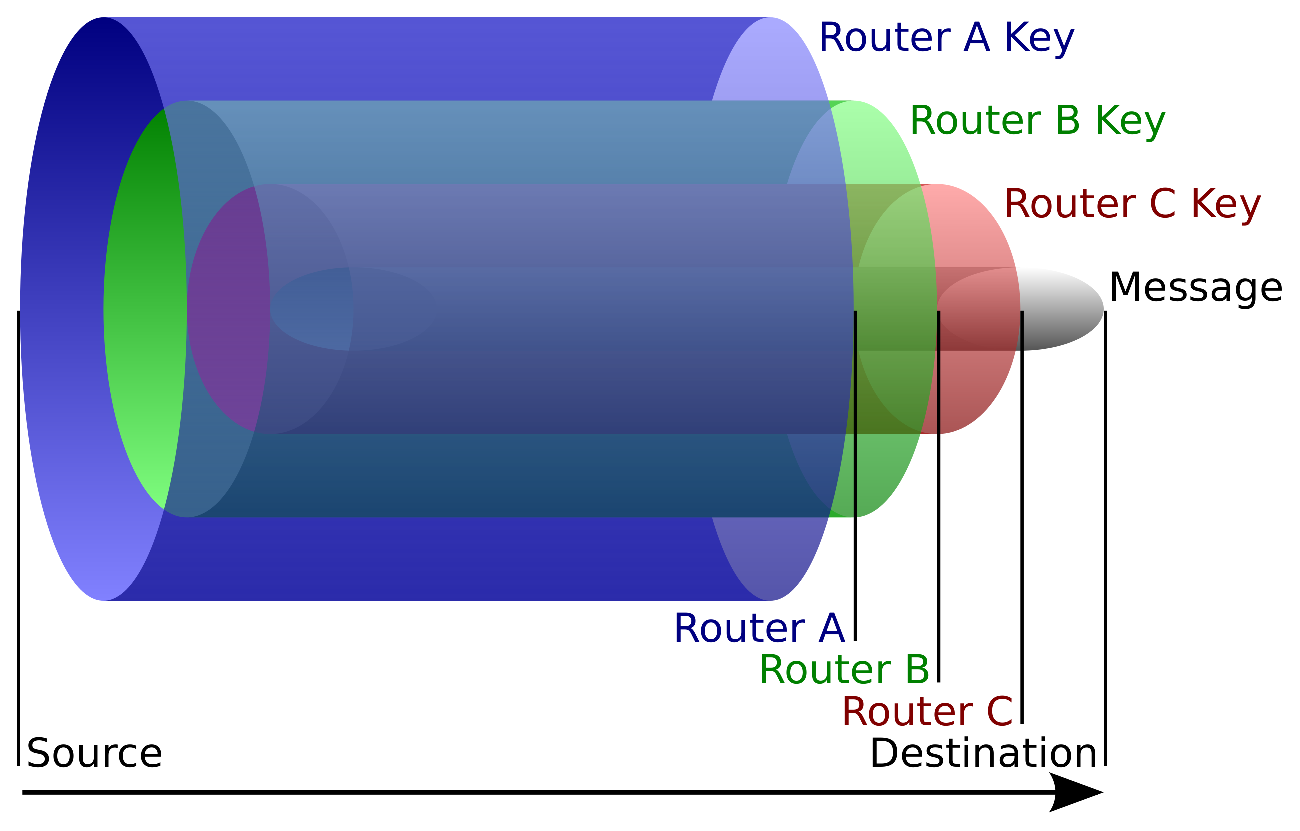
\includegraphics[width=0.5\textwidth]{images/onion-diagram.eps}
	\caption{An example cell and message encryption in an onion routing scheme. Each router ``peals'' off its respective layer of encryption; the final router exposes the final destination.}
\end{figure}

The first generation of onion routing used circuits fixed to a length of five, assumed a static network topology, and most notably, introduced the ability to mate two circuits at a common node or server. This last capability enabled broader anonymity where the circuit users were anonymous to each other and to the common server, a capability that was adopted and refined by later generation onion routers. Second generation introduced variable-length circuits, multiplexing of all user traffic over circuits, exit policies for the final router, and assumed a dynamic network by routing updates throughout the network. A client, Alice, in second-generation onion routers also distributed symmetric keys through the cell layers. If routers remember the destinations for each message they received, the recipient Bob can send his reply backwards through the circuit and each router re-encrypts the reply with their symmetric key. Alice unwraps all the layers, exposing the Bob's reply. The transition from public-key cryptography to symmetric-key encryption significantly reduced the CPU load on onion routers and enabled them to transfer more packets in the same amount of time. However, while influential, first and second generation onion routing networks have fallen out of use in favor of third-generation systems.\cite{syverson2011peel}

\section{Tor}

Tor is a third-generation onion routing system. It was invented in 2002 by Roger Dingledine, Nick Mathewson, and Paul Syverson of the Free Haven Project and the U.S. Naval Research Laboratory\cite{dingledine2004tor} and is the most popular onion router in use today. Tor inherited many of the concepts pioneered by earlier onion routers and implemented several key changes:\cite{syverson2011peel}\cite{dingledine2004tor}

\begin{itemize}
	\item \textbf{Perfect forward secrecy:} Rather than distributing keys via onion layers, Tor clients negotiate ephemeral symmetric encryption keys with each of the routers in turn, extending the circuit one node at a time. These keys are then purged when the circuit is torn down; this achieves perfect forward secrecy, a property that ensures that the encryption keys will not be revealed if long-term public keys are later compromised.
	\item \textbf{Circuit isolation:} Second-generation onion routers mixed cells from different circuits in realtime, but later research could not justify this as an effective defence against an active adversary.\cite{syverson2011peel} Tor abandoned this in favor of isolating circuits from each other inside the network. Tor circuits are used for up to 10 minutes or whenever the user chooses to rotate to a fresh circuit.
	\item \textbf{Three-hop circuits:} Previous onion routers used long circuits to provide heavy traffic mixing. Tor removed mixing and fell back to using short circuits of minimal length. With three relays involved in each circuit, the first node (the \emph{guard}) is exposed to the user's IP address. The middle router passes onion cells between the guard and the final router (the \emph{exit}) and its encryption layer exposes it to neither the user's IP nor its traffic. The exit processes user traffic, but is unaware of the origin of the requests. While the choice of middle and exits can be routers can be safely random, the guard nodes must be chosen once and then consistently used to avoid a large cumulative chance of leaking the user's IP to an attacker. This is of particular importance for circuits from hidden services.\cite{bauer2007low}\cite{overlier2006locating}
	\item \textbf{Standardized to SOCKS proxy:} Tor simplified the multiplexing pipeline by transitioning from application-level proxies (HTTP, FTP, email, etc) to a TCP-level SOCKS proxy, which multiplexed user traffic and DNS requests through the onion circuit regardless of any higher protocol. The disadvantage to this approach is that Tor's client software has less capability to cache data and strip identifiable information out of a protocol. The countermeasure was the Tor Browser, a fork of Mozilla's open-source Firefox with a focus on security and privacy. To reduce the risks of users breaking their privacy through Javascript, it ships with the NoScript extension which blocks all web scripts not explicitly whitelisted. The browser also forces all web traffic, including DNS requests, through the Tor SOCKS proxy, provides a Windows-Firefox user agent regardless of the native platform, and includes many additional security and privacy enhancements not included in native Firefox. The browser also utilizes the EFF's HTTPS Everywhere extension to re-write HTTP web requests into HTTPS whenever possible; when this happens the Tor cell contains an additional inner encryption layer.
	\item \textbf{Directory servers:} Tor introduced a set of trusted directory servers to distribute network information and the public keys of onion routers. Onion routers mirror the digitally signed network information from the directories, distributing the load. This simplified approach is more flexible and scales faster than the previous flooding approach, but relies on the trust of central directory authorities. Tor ensures that each directory is independently maintained in multiple locations and jurisdictions, reducing the likelihood of an attacker compromising all of them.\cite{syverson2011peel} We describe the contents and format of the network information published by the directories in section \ref{sec:ConsensusDocs}.
	\item \textbf{Dynamic rendezvous with hidden services:} In previous onion routers, circuits mated at a fixed common node and did not use perfect forward secrecy. Tor uses a distributed hashtable to record the location of the introduction node for a given hidden service. Following the initial handshake, the server and the client then meet at a different onion router chosen by the client. This approach significantly increased the reliability of hidden services and distributed the communication load across multiple rendezvous points.\cite{dingledine2004tor} We provide additional details on the hidden service protocol in section \ref{sec:HiddenServices} and our motivation for addition infrastructure in section \ref{sec:Motivation}.
\end{itemize}

As of March 2015, Tor has 2.3 million daily users that together generate 65 Gbit/s of traffic. Tor's network consists of nine authority nodes and 6,600 onion routers in 83 countries.\cite{TorMetrics} In a 2012 Top Secret U.S. National Security Agency presentation leaked by Edward Snowden, Tor was recognized as the "the king of high secure, low latency Internet anonymity".\cite{landau2014highlights}\cite{plak2014anonymous} In 2014, BusinessWeek claimed that Tor was ``perhaps the most effective means of defeating the online surveillance efforts of intelligence agencies around the world.''\cite{TorBusinessWeek}

\subsection{Design}

Tor's design focuses on being easily deployable, flexible, and well-understood. Tor also places emphasis on usability in order to attract more users; more user activity translates to an increased difficulty of isolating and breaking the privacy of any single individual. Tor however does not manipulate any application-level protocols nor does it make any attempt to defend against global attackers. Instead, its threat model assumes that the capabilities of adversaries are limited to observing fractions of Tor traffic, that they can actively delay, delete, or manipulate traffic, that they may attempt to digitally fingerprint packets, that they may run onion routers themselves, and that they may compromise a fraction of other existing routers. Together, most of the assumptions may be broadly classified as traffic analysis attacks. Tor's final focus is defending against these types of attacks.\cite{dingledine2004tor}

\subsection{Circuit Construction}

\begin{figure}[htdp]
	\begin{minipage}[b]{0.45\linewidth}
		\centering
		\includegraphics[width=\textwidth]{images/Tor/circuit-building-2-5.png}
		\caption{A circuit through the Tor network.}
		\label{fig:figure1}
	\end{minipage}
	\hspace{0.5cm}
	\begin{minipage}[b]{0.45\linewidth}
		\centering
		\includegraphics[width=\textwidth]{images/Tor/circuit-change-1-4.png}
		\caption{A Tor circuit is changed periodically, creating a new user identity.}
		\label{fig:figure2}
	\end{minipage}
\end{figure}

\subsubsection{Overview}

Let Alice be a client who wishes to enhance her privacy by using Tor but does not run a Tor router herself. Her basic procedure for initializing her own circuit is as follows:

\begin{enumerate}
	\item Alice selects a Tor router $ R_{1} $ and sets up an authenticated encrypted connection to it.
	\item Alice selects a second router $ R_{2} $ and tells $ R_{1} $ to build a TCP link to it. 
	\item Alice uses her $ R_{1} $ tunnel to establish an authenticated encrypted connection with $ R_{2} $.
	\item Alice selects an $ R_{3} $ and uses the $ Alice \leftrightarrow R_{1} \leftrightarrow R_{2} $ tunnel to tell $ R_{2} $ to connect to $ R_{3} $.
	\item Alice establishes an authenticates encrypted connection with $ R_{3} $ over the $ Alice \leftrightarrow R_{1} \leftrightarrow R_{2} $ tunnel.
\end{enumerate}

Following the successful circuit construction, she can then send messages out of $ R_{3} $ through the $ Alice \leftrightarrow R_{1} \leftrightarrow R_{2} \leftrightarrow R_{3} $ tunnel.

As a defense against traffic analysis using packet size, Alice packs and pads circuit traffic into equally-sized Tor \emph{cells} of 512 bytes and changes $ R_{2} $ and $ R_{3} $ every 10 minutes.\cite{mccoy2008shining}

\emph{todo: Explain why Alice must choose her guard node carefully and then stick with it.}

\subsubsection{TAP}

The Tor Authentication Protocol (TAP) is a critical piece of Tor networking infrastructure as it allows Alice to verify the authenticity of the onion routers that she selects for her circuit while still remaining anonymous herself. Namely it prevents active spoofing attacks, which if successful would deanonymize Alice and compromise her privacy.

First, TAP assumes that the following is established:

\begin{itemize}
	\item Alice has a reliable PKI that can securely distribute the identity, IP addresses, and public keys of all Tor routers. Tor accomplishes this through consensus documents from authority nodes, described in section \ref{sec:ConsensusDocs}.
	\item Let $ \mathcal{E}_{B} $ mean encryption and $ \mathcal{D}_{B} $ mean decryption under $ B $'s public-private keypair for some party $ B $.
	\item $ p $ is a prime such that $ q = \frac{q - 1}{2} $ is also prime and let $ g $ be a generator of the subgroup of $ \mathbb{Z}^{*}_{p} $ of order $ q $.
	\item Let $ R_{L} $ be a generator that returns uniformly random $ L $-bit values in the interval $ [1, \textrm{min}(q, 2 ^ L) - 1] $.
	\item Define $ f $ as SHA-1 which takes input from $ \mathbb{Z}_{p} $ and returns a $ L_{f} $-bit value.
\end{itemize}

\emph{Todo: I'd like to include that TAP diagram \cite{ling2013protocol}\cite{dingledine2004tor} and find out about the forward-backwards keys.}

Then TAP proceeds as:

\begin{enumerate}
	\item \label{item:First1}
		\begin{enumerate}
			\item Alice selects a Tor router, $ R_{i} $.
			\item Alice generates $ x = R_{L} $ and computes $ s = g ^ x \bmod{p} $.
			\item Alice sends $ c = \mathcal{E}_{R_{i}}(s) $ to $ R_{i} $.
		\end{enumerate}
	\item
		\begin{enumerate}
			\item $ R_{i} $ computes $ m = \mathcal{D}_{R_{i}}(c) $ and confirms that $ 1 < m < p - 1 $.
			\item $ R_{i} $ generates $ y = R_{L} $ and computes $ a = g ^ y \bmod{p} $ and $ b = f(m ^ y \bmod{p}) $.
			\item $ R_{i} $ sends $ (a, b) $ to Alice.
		\end{enumerate}
	\item
		Alice confirms that $ 1 < a < p - 1 $ and that $ b = f(a ^ x \bmod{p}) $.
	\item \label{item:Last1}
		If the assertions pass, then Alice has confirmed $ R_{i} $'s identity and now Alice and $ R_{i} $ can use $ a ^ x = m ^ y $ as a shared symmetric encryption key and encrypt messages under AES.
	\item 
		Alice repeats steps \ref{item:First1} -- \ref{item:Last1} until the circuit is of the desired length.
\end{enumerate}

Thus for each router in the circuit, Alice perform one public-key encryption and her half of a Diffie-Hellman-Merkle (DHE) handshake, and each router in turn performs one private-key decryption and their half of a DHE handshake. Under the assumptions that RSA is one way, AES remains unbroken, and $ f $ is strong and acts as a random oracle, an attacker has only a negligible chance of being able to impersonate $ R_{i} $ and read messages that she tunnels through the circuit.\cite{goldberg2006security}

\subsubsection{NTor}

%tense changes

In mid 2013, TAP was superseded by ``NTor'', a new protocol invented by Goldberg, Stebila, and Ustaoglu.\cite{goldberg2013anonymity} Compared to TAP, NTor replaced the computational cost associated with DHE exponentiation with significantly more efficient elliptic curve cryptography (ECC). Its implementation uses Curve25519,\cite{bernstein2006curve25519} a Montgomery curve designed by Bernstein to be used for high-speed ECDHE key exchanges. All Curve25519 operations are implemented to run in $ \mathcal{O}(1) $ time.

NTor is initialized by defining the following,

\begin{itemize}
	\item Let $ H(x,k) $ be HMAC-SHA256, which accepts a message $ x $ and yield a 32-byte MAC output. Let $ k_{1} $, $ k_{2} $, and $ k_{3} $ be some fixed secret keys for the HMAC algorithm, $ k_{1} \neq k_{2} \neq k_{3} $.
	%\item Let $ \mathit{C}_{\mathit{pub}}(basept, pvt) $ yield a 32-byte Curve25519 public key given a base point $ basept $ and a private key $ pvt $.
	\item Let $ \mathit{C}_{\mathit{gen}}() $ generate a Curve25519 keypair. This function requires 32 bytes from a cryptographically secure source (such as a CSPRNG) to generate the private key, then it derives the public key.
	\item Let $ \mathit{C}_{\mathit{sec}}(pvt, pub) $ yield a 32-byte common secret given a Curve25519 private and public key, $ pvt $ and $ pub $, respectively.
	%\item Let $ K_{\mathit{gen}} $ yield $ a $ and $ A $, the private and public halves, respectively, of the Curve25519 keypair.
	\item Let each Tor router $ R_{j} $ generate $ b_{j},B_{j} = \mathit{C}_{\mathit{gen}}() $ and publish $ B_{j} $ through the consensus document.
	\item Let $ \mathit{id} $ by the router's identification fingerprint.
\end{itemize}

Then NTor proceeds as:

\begin{enumerate} % 216-ntor-handshake.txt
	\item \label{item:First2}
		\begin{enumerate}
			\item Alice selects a Tor router, $ R_{i} $.
			\item Alice generates $ x,X = C_{\mathit{gen}}() $ and sends $ X $ to $ R_{i} $.
		\end{enumerate}
	\item
		\begin{enumerate}
			\item $ R_{i} $ generates $ y,Y = C_{\mathit{gen}}() $.
			\item $ R_{i} $ sets $ \mathit{sec} = C_{\mathit{sec}}(y, X) \concat C_{\mathit{sec}}(b, X) \concat \mathit{id} \concat X \concat Y $.
			\item $ R_{i} $ computes $ \mathit{seed} = H(\mathit{sec, k_{1}}) $.
			\item $ R_{i} $ computes $ \mathit{auth} = H(H(\mathit{sec, k_{2}}) \concat id \concat B \concat Y \concat X, k_{3}) $.
			\item $ R_{i} $ sends $ Y $ and $ \mathit{auth} $ to Alice.
			\item $ R_{i} $ deletes the $ y,Y $ keypair.
		\end{enumerate}
	\item
		\begin{enumerate}
			\item Alice sets $ \mathit{sec} = C_{\mathit{sec}}(x, Y) \concat C_{\mathit{sec}}(x, B) \concat \mathit{id} \concat X \concat Y $.
			\item Alice computes $ \mathit{seed} = H(\mathit{sec, k_{1}}) $.
			\item Alice confirms that $ \mathit{auth} = H(H(\mathit{sec, k_{2}}) \concat id \concat B \concat Y \concat X, k_{3}) $.
		\end{enumerate}
	\item
		Alice and $ R_{i} $ now have a shared secret $ \mathit{seed} $ that is then used indirectly for symmetric key encryption.	
\end{enumerate}

\subsection{Consensus Documents}
\label{sec:ConsensusDocs}

\emph{Todo: this section is incomplete. Here I plan to detail the consensus documents that I will be using, since I use them in my Solution section.}

The Tor network is maintained by nine authority nodes, who each vote on the status of nodes and together hourly publish a digitally signed consensus document containing IPs, ports, public keys, latest status, and capabilities of all nodes in the network. The document is then redistributed by other Tor nodes to clients, enabling access to the network. The document also allows clients to authenticate Tor nodes when constructing circuits, as well as allowing Tor nodes to authenticate one another. Since all parties have prior knowledge of the public keys of the authority nodes, the consensus document cannot be forged or modified without disrupting the digital signature.\cite{xin2009design}

\subsubsection{cached-certs}

\emph{This section is incomplete. See https://collector.torproject.org/formats.html}

\subsubsection{cached-microdescs}

\emph{This section is incomplete. See Tor's dir-spec.txt, section 3.3}

\subsubsection{cached-microdesc-consensus}

\emph{This section is incomplete. See https://collector.torproject.org/formats.html}

\subsection{Hidden Services}
\label{sec:HiddenServices}

Although Tor's primary and most popular use is for secure access to the traditional Internet, Tor also supports \emph{hidden services} -- anonymous servers hosting services such as websites, marketplaces, or chatrooms. These servers intentionally mask their IP addresses through Tor circuits and thus cannot normally be accessed outside the context of Tor. In contrast to Tor-anonymized web requests where the client is anonymous but the server is known, Tor hidden services provide bidirectional anonymity where both parties remain anonymous and never directly communicate with one another.\cite{nicolussi2011human}

Tor does not contain a DNS system for its websites; instead hidden service addresses are algorithmically generated by generating the SHA-1 hash of their public RSA key, truncating to 80 bits, and converting the remainder to base58. Ignoring the possibility of SHA-1 collisions, this builds a one-to-one relationship between a hidden service's public key and its address which can be confirmed without requiring any identifiable information or central authorities. The address is the appended with the .onion Top-Level Domain (TLD).

A hidden server, Bob, first builds Tor circuits to several random relays and enables them to act as \textit{introduction points} by giving them its public key, $ B_{K} $. He then then uploads his public key and the fingerprint identity of these nodes to a distributed hashtable inside the Tor network, signing the result. He then publishes his hidden service address in a backchannel. When Alice obtains this address and enters it into a Tor-enabled browser, her software queries this hashtable, obtains $ B_{K} $ and Bob's introduction points, and builds a Tor circuit to one of them, $ ip_{1} $. Simultaneously, the client also builds a circuit to another relay, $ rp $, which she enables as a rendezvous point by telling it a one-time secret, $ sec $. During this procedure, hidden services must continue to use their same entry node in order to avoid leaking its IP address to possibly malicious onion routers.\cite{bauer2007low}\cite{overlier2006locating}

\begin{figure}[htdp]
	\begin{minipage}[b]{0.45\linewidth}
		\centering
		\includegraphics[width=\textwidth]{images/Tor/tor-hidden-service-4-higher.png}
		\caption{Alice uses the encrypted cookie to tell Bob to switch to $ rp $.}
	\end{minipage}
	\hspace{0.5cm}
	\begin{minipage}[b]{0.45\linewidth}
		\centering
		\includegraphics[width=\textwidth]{images/Tor/tor-hidden-service-6.png}
		\caption{Bidirectional communication between Alice and the hidden service.}
	\end{minipage}
\end{figure}

She then sends to $ ip_{1} $ a cookie encrypted with $ B_{K} $, containing $ rp $ and $ sec $. Bob decrypts this message, builds a circuit to $ rp $, and tells it $ sec $, enabling Alice and Bob to communicate. Their communication travels through six Tor nodes: three established by Alice and three by Bob, so both parties remain anonymous. From there traditional HTTP, FTP, SSH, or other protocols can be multiplexed over this new channel.

As of March 2015, Tor hosts approximately 25,000 unique hidden services that together generate around 450 Mbit/s of traffic.\cite{TorMetrics}

\section{Motivation}
\label{sec:Motivation}

As Tor's hidden service addresses are algorithmically derived from the service's public RSA key, there is at best limited capacity to select a human-meaningful name. Some hidden service operators have attempted to work around this issue by finding an RSA key by brute-force that generates a partially-desirable hidden service address (e.g. ``example0uyw6wgve.onion'') and although some alternative encoding schemes have been proposed, (section \label{sec:EncodingSchemes}) the problem generally remains. The usability of hidden services is severely challenged by their non-intuitive and unmemorable base58-encoded domain name. For example, 3g2upl4pq6kufc4m.onion is the address for the DuckDuckGo search engine, \\ suw74isz7wqzpmgu.onion is a WikiLeaks mirror, and 33y6fjyhs3phzfjj.onion and \\ vbmwh445kf3fs2v4.onion are both SecureDrop instances for anonymous document submission. These addresses maintain strong privacy as the strong association between its public key and its address significantly breaks the association between the service's purpose and its address. However, this privacy comes at a cost: it is impossible to classify or label a hidden service's purpose in advance, a fact well known within Tor hidden service communities. Over time, third-party directories -- both on the Clear and Dark Internets -- appeared in attempt to counteract this issue, but these directories must be constantly maintained and furthermore this approach is not convenient nor does it scale well. This suggests the strong need for a more complete and reliable solution.

\section{Contributions}

Our contribution to this problem is six-fold:

\begin{itemize}
	\item We introduce a novel distributed naming system that enables Tor hidden service operators to choose a unique human-meaningful domain name and construct a strong association between that domain name and their hidden service address, squaring Zooko's Triangle (section \ref{sec:ZookosTriangle}).
	\item We described a new distributed, publicly confirmable, and partially self-healing transactional database.
	\item We provide OnioNS as a Tor plugin and rely on the existing Tor network and other infrastructure, rather than introduce a new network. This simplifies our assumptions and reduces our threat model to attack vectors already known and well-understood on the Tor network.
	\item We introduce a novel protocol for proving the non-existence of any domain name.
	\item We enable Tor clients to verify the authenticity of a domain name against its corresponding hidden service address with minimal data transfers and without requiring any additional queries.
	\item We preserve the privacy of both the hidden service and the anonymity of Tor clients connecting to it.
\end{itemize}

	
\chapter{\uppercase{Background}}

\section{Tor}

The Tor network is a third-generation onion routing system, originally designed by the U.S. Naval Research Laboratory for protecting sensitive government communication, but today it continues to see global widespread use. Tor refers both to the client-side multiplexing software and to the worldwide volunteer-run network of over six thousand nodes. The Tor software provides an anonymity and privacy layer to end-users by relaying TCP traffic through a series of relays on the Tor network. Tor's encryption and routing protocols are designed to make it very difficult for an adversary to correlate an end user to their traffic. Tor has been recognized by the NSA as the "the king of high secure, low latency Internet anonymity".

\subsection{Design}

Tor routes encrypted TCP/IP user traffic through a worldwide volunteer-run network of over six thousand relays. Typically this route consists of a carefully-constructed three-hop path known as a \textit{circuit}, which changes over time. These nodes in the circuit are commonly referred to as \textit{guard node}, \textit{middle relay}, and the \textit{exit node}, respectively. Only the first node is exposed to the origin of TCP traffic into Tor, and only the exit node can see the destination of traffic out of Tor. The middle router, which passes encrypted traffic between the two, is unaware of either. The client negotiates a separate TLS connection with each node at a time, and traffic through the circuit is decrypted one layer at a time. As such, each node is only aware of the machines it talks to, and only the client knows the identity of all three nodes used in its circuit, making traffic correlation much more difficult difficult compared to a VPN, proxy, or a direct TLS connection.

The Tor network is maintained by nine authority nodes, who each vote on the status of nodes and together hourly publish a digitally signed consensus document containing IPs, ports, public keys, latest status, and capabilities of all nodes in the network. The document is then redistributed by other Tor nodes to clients, enabling access to the network. The document also allows clients to authenticate Tor nodes when constructing circuits, as well as allowing Tor nodes to authenticate one another. Since all parties have prior knowledge of the public keys of the authority nodes, the consensus document cannot be forged or modified without disrupting the digital signature.\cite{Xin2009}

\subsection{Routing}

In traditional Internet connections, the client communicates directly with the server. TLS encryption cannot hide IP and TCP headers, which must be exposed to allow routing. Eeavesdroppers can track end-users by monitoring these headers, easily correlating clients to the their activities. Tor combats this by routing end user traffic through a randomized circuit through the network of relays. The client software first queries an authority node or a known relay for the latest consensus document. Next, the Tor client chooses three unique and geographically diverse nodes to use. It then builds and extends the circuit one node at at time, negotiating respective TLS connections with each node in turn. No single relay knows the complete path, and each relay can only decrypt its layer of decryption. In this way, data is encrypted multiple times and then is decrypted in an onion-like fashion as it passes through the circuit.

\begin{figure}[htdp]
	\begin{minipage}[b]{0.45\linewidth}
		\centering
		\includegraphics[width=\textwidth]{images/circuit-construction.png}
		\caption{Anatomy of the construction of a Tor circuit.}
		\label{fig:figure1}
	\end{minipage}
	\hspace{0.5cm}
	\begin{minipage}[b]{0.45\linewidth}
		\centering
		\includegraphics[width=\textwidth]{images/circuit-building-2-5.png}
		\caption{A circuit through the Tor network.}
		\label{fig:figure2}
	\end{minipage}
\end{figure}

The client first establishes a TLS connection with the first relay, $R_{1}$, using the relay's public key. The client then performs an ECDHE key exchange to negotiate $K_{1}$ which is then used to generate two symmetric session keys: a forward key $K_{1,F}$ and a backwards key $K_{1,B}$. $K_{1,F}$ is used to encrypt all communication from the client to $R_{1}$ and $K_{1,B}$ is used for all replies from $R_{1}$ to the client. These keys are used conjunction with the symmetric cipher suite negotiated during the TLS handshake, thus forming an encrypted tunnel with perfect forward secrecy. Once this one-hop circuit has been created, the client then sends $R_{1}$ the RELAY\_EXTEND command, the address of $R_{2}$, and the client's half of the Diffie-Hellman-Merkle protocol using $K_{1,F}$. $R_{1}$ performs a TLS handshake with R${2}$ and uses $R_{2}$'s public key to send this half of the handshake to $R_{2}$, who replies with his second half of the handshake and a hash of $K_{2}$. $R_{1}$ then forwards this to the client under $R_{1,B}$ with the RELAY\_EXTENDED command to notify the client. The client generates $K_{1,F}$ and $K_{1,B}$ from $K_{2}$, and repeats the process for $R_{3}$,\cite{Ling2012} as shown in Figure 3. The TCP/IP connections remain open, so the returned information travels back up the circuit to the end user.

Following the complete establishment of a circuit, the Tor client software then offers a Secure Sockets (SOCKS) interface on localhost which multiplexes any TCP traffic through Tor. At the application layer, this data is packed and padded into equally-sized Tor \textit{cells}, transmission units of 512 bytes. As each relay sees no more than one hop in the circuit, in theory neither an eavesdropper nor a compromised relay can link the connection's source, destination, and content. Tor further obfuscates user traffic by changing the circuit path every ten minutes,\cite{McCoy2008} as shown in Figure 4. A new circuit can also be requested manually by the user.

\begin{figure}[htbp]
	\centering
	\includegraphics[width=0.6\textwidth]{images/circuit-change-1-4.png}
	\caption{A Tor circuit is changed periodically, creating a new user identity.}
	\label{fig:figure3}
\end{figure}

% Although a different guard node is used here, in practice the choice of entry point is preserved for extended periods of time.

Tor users typically use the Tor Browser, a custom build of Mozilla Firefox with a focus on security and privacy. The TBB anonymizes and provides privacy to the user in many ways. These include blocking all web scripts not explicitly whitelisted, forcing all traffic including DNS requests through the Tor SOCKS port, mimicking Firefox in Windows both with a user agent (regardless of the native platform) and SSL cipher suites, and reducing Javascript timer precision to avoid identification through clock skew. Furthermore, the TBB includes the Electronic Frontier Foundation's HTTPS Everywhere extension, which uses regular expressions to rewrite HTTP web requests into HTTPS for domains that are known to support HTTPS. If this is the case, an HTTPS connection will be established with the web server. If this happens, end-to-end encryption is complete and an outsider near the user would be faced with up to four layers of TLS encryption: $K_{1,F}(K_{2,F}(K_{3,F}(K_{server}(\textrm{client\ request}))))$ and likewise $K_{1,B}(K_{2,B}(K_{3,B}(K_{server}(\textrm{server\ reply}))))$ for the returning traffic, making traffic analysis very difficult.

\subsection{Hidden Services}

Although Tor's primary and most popular use is for secure access to the traditional Internet, Tor also supports anonymous services, such as websites, marketplaces, or chatrooms. These are a part of the Dark Web and cannot be normally accessed outside the context of Tor. In contrast to Tor-anonymized web requests where the client is anonymous but the server is known, Tor hidden services provide bidirectional anonymity where both parties remain anonymous and never directly communicate with one another. This allows for a greater range of communication capabilities. Tor's hidden service protocol was introduced in 2004 and has not seen a major revision since then.\cite{NicolussiThesis2011}

Tor hidden services are known only by their public RSA key. Tor does not contain a DNS system for its websites; instead the domain names of hidden services are an 80-bit truncated SHA-1 hash of its public key, postpended by the .onion Top-Level Domain. Once the hidden service is contacted and its public key obtained, this key can be checked against the requested domain to verify the authenticity of the service server. This process is analogous to SSL certificates in the clearnet, however Tor's authenticity check leaks no identifiable information about the anonymous server. If a client obtains the hash domain name of the hidden service through a backchannel and enters it into the Tor Browser, the hidden service lookup begins.

Preceding any client communication, the hidden server, Bob, first builds Tor circuits to several random relays and enables them to act as \textit{introduction points} by giving them its public key, $B_{K}$. The server then uploads its public key and the fingerprint identity of these nodes to a distributed hashtable inside the Tor network, signing the result. When a client, Alice, requests contact with Bob, Alice's Tor software queries this hashtable, obtains $B_{K}$ and Bob's introduction points, and builds a Tor circuit to one of them, $IP_{1}$. Simultaneously, the client also builds a circuit to another relay, $RP$, which she enables as a rendezvous point by telling it a one-time secret, $S$.

\begin{figure}[htdp]
	\begin{minipage}[b]{0.45\linewidth}
		\centering
		\includegraphics[width=\textwidth]{images/tor-hidden-service-4-higher.png}
		\caption{Alice uses the encrypted cookie to tell Bob to switch to $RP$.}
		\label{fig:figure4}
	\end{minipage}
	\hspace{0.5cm}
	\begin{minipage}[b]{0.45\linewidth}
		\centering
		\includegraphics[width=\textwidth]{images/tor-hidden-service-6.png}
		\caption{Bidirectional communication between Alice and the hidden service.}
		\label{fig:figure5}
	\end{minipage}
\end{figure}

She then sends to $IP_{1}$ an cookie encrypted with $B_{K}$, containing $RP$ and $S$. Bob decrypts this message, builds a circuit to $RP$, and tells it $S_{1}$, enabling Alice and Bob to communicate. Their communication travels through six Tor nodes: three established by Alice and three by Bob, so both parties remain anonymous. From there traditional HTTP, FTP, SSH, or other protocols can begin, multiplexed over this new channel.

\section{Motivation}

The usability of hidden services is severely challenged by their non-intuitive 16-character hexadecimal domain names: 3g2upl4pq6kufc4m.onion is the address for the DuckDuckGo hidden service, whereas 33y6fjyhs3phzfjj.onion is the Guardian's SecureDrop service for anonymous document submission, and blockchainbdgpzk.onion is the anonymized edition of blockchain.info. It is rarely clear what service a hidden server is providing by its domain name alone without relying on third-party directories for the correlation, directories which must be updated and reliably maintained constantly. These must be then distributed through backchannels such as /r/onions, the-hidden-wiki.com, or through a hidden service that is known in advance.

One attempt at alleviating the issue is to generate hidden service many RSA keys in an attempt to find one whose hash contains or begins with a meaningful name. This is the case with Blockchain.info's hidden service, although such attempts are time-consuming and only partially effective because the size of the domain keyspace is too large to be effectively brute-forced in any reasonable length of time. Tor Proposal 224 makes this solution even worse as it suggests 32-byte domain names which embed the entire hidden service key in base32. Although prefixing the domain name with a meaningful word helps identify a hidden service, it does nothing to alleviate the logistic problems of entering a hidden service domain name manually into the Tor Browser, an issue that is not shared by domains in the clearnet.

It is clear that the usability problem exists and none of the few attempts to solve it have been fully successful. It is for these reasons that I propose EsgalDNS as a full solution.

	
\chapter{\uppercase{Requirements}}

\section{Assumptions and Threat Model}

One of the primary assumptions that I make in this system is that not all Tor nodes can be trusted. Some of them may be run by malicious operators, curious researchers, or experimenting developers. They may be wiretapped, the Tor software modified and recompiled, or they may otherwise behave in an abnormal fashion. I assume that adversaries have control over some of the Tor network, they have access to large amounts of computational and financial resources, and that they have access to portions of Internet traffic, including portions of Tor traffic. I also assume that they do not have global and total Internet monitoring capabilities and I make no attempt to defend against such an attacker, although it should be noted that neither does Tor. I work under the believe that attackers are not capable of cryptographically breaking properly-executed TLS connections and their modern components, particularly the AES cipher, ECDHE key exchange, and the SHA2 series of digests, and that they maintain no backdoors in the Botan and OpenSSL implementations of these algorithms. Lastly, I assume that adversaries monitor and may attempt to modify the DNS record databases, but I assume that at least 50 percent of the Tor network is trustworthy and behave normally in accordance with Tor specifications.

\section{Design Principles}

Tor's high security environment is challenging to the inclusion of additional capabilities, even to systems that are backwards compatible to existing infrastructure. Anonymity, privacy, and general security are of paramount importance. We enumerate a short list of requirements for any secure DNS system designed for safe use by Tor clients. We later show how existing works do not meet these requirements and how we overcome these challenges with EsgalDNS.

\begin{enumerate}
	\item The registrations must be anonymous; it should be infeasible to identify the registrant from the registration, including over the wire.
	\item Lookups must be anonymous; clients must stay anonymous when looking up registrations, otherwise they leak what hidden services they are interested in.
	\item Registrations must be publicly confirmable; clients must be able to verify that the registration came from the desired hidden service and that the registration is not a forgery.
	\item Registrations must be securely unique, or have an extremely high chance of being securely unique such as when this property relies on the collision-free property of cryptographic hashes.
	\item It must be distributed. The Tor community will adamantly reject any centralized solution for Tor hidden services for security reasons, as centralized control makes correlations easy, violating our first two requirements.
	\item It must remain simple to use. Usability is key as most Tor users are not security experts. Tor hides non-essential details like routing information behind the scenes, so additional software should follow suite.
	\item It must remain backwards compatible; the existing Tor infrastructure must still remain functional.
	\item It should not be feasible to maliciously modify or falsify registrations in the database or in transit, even though insider attacks.
\end{enumerate}

The current Tor hidden service protocol meets the first, second, and sevenths requirements though the use of Tor circuits, the third by the nature of the hidden service domain names, the fourth because of the collision-free property of SHA-1, the fifth due to the hashtable in the Tor network, and the eight requirement because of the verifiability of the domain names to the service's public keys. However, it only partially meets the sixth requirement because although the domain names are entered in the traditional manner into the Tor Browser, the domain names are not entirely human-meaningful or memorable so it suffers from usability problems. 

Several additional objectives, although they are not requirements, revolve around performance: it should be assumed that it is impractical for clients to download the entirety or large portions of the domain database in order to verify any of the requirements, a DNS system should take a reasonable amount of time to resolve domain name queries, and that the system should not incur any significant load on client computers.
	

\chapter{\uppercase{Challenges}}

\section{Zooko's Triangle}

One of the largest challenges is inherent to the difficulty of designing a distributed system that maintains a correlation database of human-meaningful names in a one-to-one fashion. The problem is summarized in Zooko's Triangle, an influential conjecture proposed by Zooko Wilcox-O'Hearn in late 2001. The conjecture states that in a persistent naming system, only two out of the three following properties can be established:\cite{Ferdous2009}

\begin{itemize}
  \item Human meaningfulness: the names have a quality of meaningfulness and memorability to the users. 
  \item Securely one-to-one: each name is unique, corresponds to a unique entity or owner, and cannot be forged.
  \item Distributed: the naming system lacks a central authority or database for allocating and distributing names.
\end{itemize}

\begin{figure}[htbp]
	\centering
	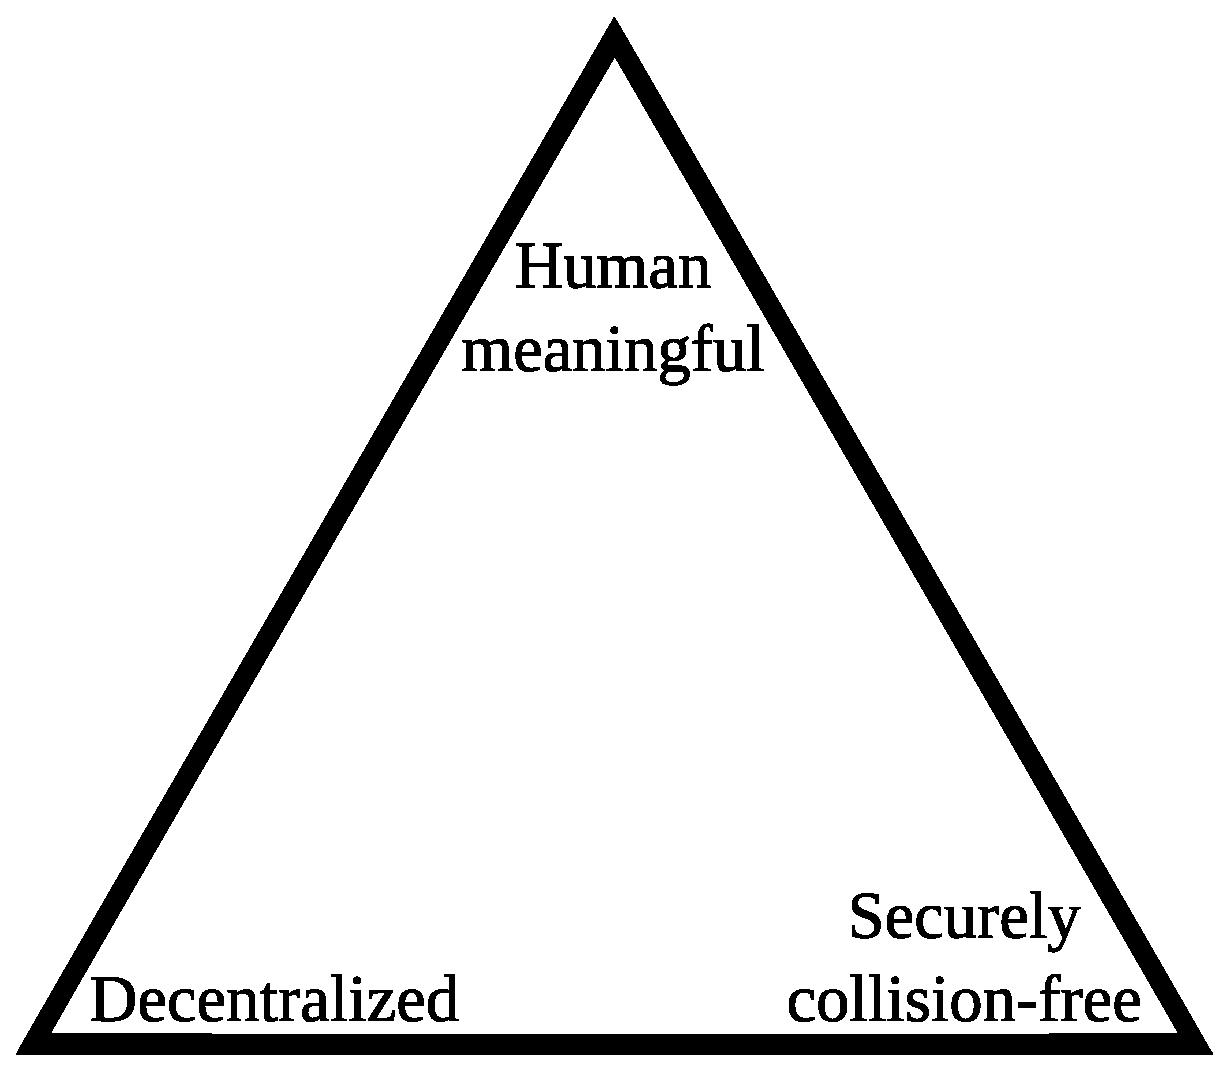
\includegraphics[width=0.3\textwidth]{images/Zooko.eps}
	\caption{Zooko's Triangle.}
	\label{fig:figure8}
\end{figure}

For example, Tor hidden service .onion addresses and Bitcoin addresses are secure and decentralized but are not human-meaningful. Clearnet domain names are memorable and provably collision-free, but use central database managed DNS under the jurisdiction of ICANN. Finally, human nicknames are meaningful and distributed, but not securely collision-free.\cite{Stiegler2005}

In recent years, systems have been developed that have shown Zooko's Triangle to be false. One prominent example is Namecoin, a naming system which uses a Bitcoin-like blockchain to store name-value pairs. Human-meaningful names can be embedded in the blockchain, which is distributed by nature. The uniqueness of the names is ensured by the Namecoin network and can be verified with anyone holding the blockchain. However, Tor developers have been wary of using Namecoin to store domain names for Tor hidden services. It is also impractical to require all Tor clients to download the entire blockchain before being able to use a hidden service DNS system, and there are inherent security challenges involved with querying servers or the Namecoin network for a registration without being able to use a complete blockchain to verify it. Therefore, another solution is needed.
	

\chapter{\uppercase{Existing Works}}

Existing literature proposing DNS systems for Tor is fairly sparse, though some ideas have been put forward.

\section{Clearnet DNS}

The Internet Domain Name Service (DNS) is a hierarchical distributed naming system for computers connected to the Internet. It links two principal Internet namespaces, Internet Protocol (IP) addresses and domain names, and translates one to the other. IP addresses specify the location of a computer or device on a network and domain names identify that resource. Domain names also serve as an abstraction layer so that devices can be moved to a different physical location or to a different IP address without loss of functionality. In contrast to IP addresses, domain names are human-meaningful and easily memorized, so DNS is a crucial component to the usability of the Internet.

Domain names on the Internet consist of a sequence of labels, delimited by dotes. The right-most label is the top-level domain (TLD) and can be used to classify the Internet resource by country or by organization type, although generic TLDs are more common. One or more subdomains follow the TLD. Each label can consist of up to 63 characters and the domain names can be up to 253 characters.



\section{Namecoin}

% TODO: expand: I spend six pages on Tor + hidden services, I should spend six pages on BTC + Namecoin, and two on DNS
% question: I'm aiming for 50 pages, and it looks I'll be burning 14 or 15 on introductions. Is that all right? If not, reduce to 5 + 5 + 1

Bitcoin is a decentralized peer-to-peer digital cryptocurrency, created by pseudonymous developer Satoshi Nakamoto in 2008. Ownership of Bitcoins consists of holding a private ECDSA key, and a transfer is a transmission of Bitcoins from one key to another. All transactions are recorded on a public ledger, called a blockchain, a data structure whose integrity is ensured through computational power but publically verifiable. Bitcoins are generated computationally at a fixed rate by \textit{miners} in a process that also secures the blockchain. Although Bitcoin received limited attention in the first two years of its life, it has since grown significantly since then, with approximately 70,000 daily transactions as of the time of this writing. Bitcoin's growth has led to the creation of many alternative cryptocurrencies, and its popularity has influenced financial discussions and legal controversy worldwide.

\subsection{Architecture}

A blockchain is data structure fundamental to Bitcoin, and crucial for its functionality. As a distributed decentralized system, this public ledger is Nakamoto's answer to the problem of ensuring agreement of critical data across all involved parties. The blockchain is a novel structure, and its structure guarantees integrity, chronological ordering of transactions, and the prevention of double-spending of Bitcoins. The blockchain consists of blocks of data that are held together by proof-of-work, a cryptographic puzzle whose solution is provably hard to find but trivial to verify. Bitcoin's proof-of-work is based on Adam Back's Hashcash scheme: that is, find a nonce such that the hash of this nonce and some data produces a result that begins with a certain number of zero bits. In Bitcoin's case this is stated as finding a nonce that when passed through two rounds of SHA256 ($ \textrm{SHA}256^{{2}} $) produces a value less than or equal to a target $ T $. This requires a party to perform on average $ \frac{1}{Pr[H \leq T]} = \frac{2 ^ {{256}}}{T} $ amount of computations, but it is easy to verify that $ \textrm{SHA}256^{{2}}(\textrm{msg} || n) \leq T $. Nodes in the Bitcoin network collectively agree to use the blockchain with the highest accumulation of computational effort, so an adversary seeking to modify the structure would need to recompute the proof-of-work for all previous blocks as well as out-perform the network, which is currently considered infeasible.\cite{Okupski2014}

Each block in the blockchain consists of a header and a payload. The header contains a hash of the previous block's header, the root hash of the Merkle tree built from the transactions in this block, a timestamp, a target $ T $, and a nonce. The block payload consists of a list of transactions. The root node of the Merkle tree ensures the integrity of the transaction vector: verifying that a given transaction is contained in the tree takes $ log(n) $ hashes, and a Merkle tree can be built $ n * log(n) $ time, ensuring that all transactions are accounted for. The hash of the previous block in the header ensures that blocks are ordered chronologically, and the Merkle root hash ensures that the transactions contained in each block are order chronologically as well. The target $ T $ changes every 2016 blocks in response to the speed at which the proof-of-work is solved such that Bitcoin miners take two weeks to generate 2016 blocks, or one block every 10 minutes. The $ \textrm{SHA}256^{{2}} $ proof-of-work provides integrity of the data structure, and secp256k1 ECDSA key are used to prove ownership of coins.\cite{Okupski2014}

\begin{figure}[htbp]
	\centering
	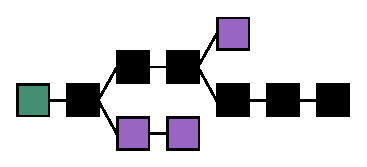
\includegraphics[width=0.6\textwidth]{images/Blockchain-2.eps}
	\caption{A sample blockchain.}
	\label{fig:figure6}
\end{figure}

\begin{figure}[htbp]
	\centering
	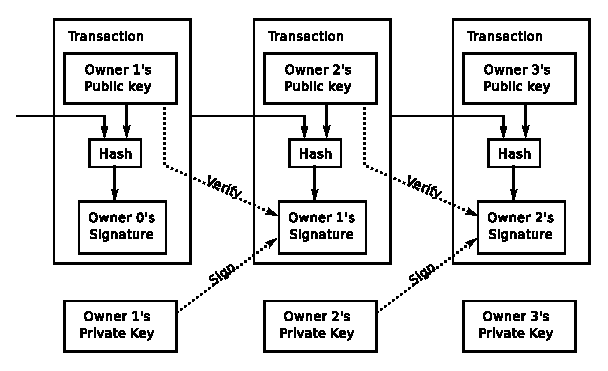
\includegraphics[width=0.6\textwidth]{images/bitcoin_transaction.eps}
	\caption{Three traditional Bitcoin transactions.}
	\label{fig:figure7}
\end{figure}

In the possibility that multiple nodes solve the proof-of-work and generate a new block simultaneously, the block becomes orphaned, the transactions recycled, and the blockchain follows the longest path from the genesis node to the latest block. Each transaction contains the public of the recipient, the ECDSA digital signature of the transaction from the sender, and the hash of the originating transaction. In this way, the digital signatures and proof-of-work in the blockchain can be traced back to the origin and forwards indefinitely. %In practice transactions can contain multiple input and outputs.

In recent years, systems have been developed that have shown Zooko's Triangle to be false. One prominent example is Namecoin, a naming system which uses a Bitcoin-like blockchain to store name-value pairs. Human-meaningful names can be embedded in the blockchain, which is distributed by nature. The uniqueness of the names is ensured by the Namecoin network and can be verified with anyone holding the blockchain. However, Tor developers have been wary of using Namecoin to store domain names for Tor hidden services. It is also impractical to require all Tor clients to download the entire blockchain before being able to use a hidden service DNS system, and there are inherent security challenges involved with querying servers or the Namecoin network for a registration without being able to use a complete blockchain to verify it. Therefore, another solution is needed.

Namecoin is a decentralized information registration and transfer system based on Bitcoin. It was the first software fork of Bitcoin and was introduced in April 2011. It uses its own blockchain and can hold name-value pairs in the blockchain attached to coins. While Bitcoin is primarily focused on supporting a currency, Namecoin aims to be a general key-value store, capable of holding cryptographic keys, DNS registrations, or other arbitrary data. It is most commonly used as a secure and censorship-resistance replacement for clearnet DNS. In 2014, Namecoin was recognized by ICANN is the most well-known example of a PKI and DNS system with an emphasis of distributed control and privacy, a growing trend in light of the revelations about the US Government by Edward Snowden. %https://www.icann.org/en/system/files/files/report-21feb14-en.pdf

\subsection{Names}

Although it inheriting Bitcoin's existing infrastructure, Namecoin added several transaction types specifically for registering and processing names, along with two new rules: names in the blockchain expire after 36,000 blocks unless renewed by the owner and no two unexpired names can be identical. These rules are enforced in the blockchain by Namecoin nodes and anyone verifying the Namecoin blockchain. Registering a name consumes 0.01 Namecoin, names can also be transferred to other owners, and they are two types: DNS and personal. The DNS type uses a new Top Level Domain (TLD) not in use by ICANN: .bit, and is used for DNS registrations. The personal name can contain arbitary data, including user information such as cryptographic keys. Like Bitcoin, Namecoin's maximum block size is one megabyte and the difficulty is set such that blocks generate every 10 minutes. Thus names expire every 250 days. 





\section{Different Encoding}

One of the most prominent is a 2011 Bachelor's thesis which outlines representing a hidden service's domain name as a series of words, rather than a base58-encoded hash.\cite{NicolussiThesis2011} However, while this scheme would improved recognition and memorability of hidden services, the words would remain random, are not chosen in advance, and do not relate to the hidden service in any meaningful way. Therefore this solution is an improvement but is not a solution. The problem remains open.
	

\chapter{\uppercase{Solution}}

\section{Overview}

I propose a new DNS system for Tor hidden services, which I am calling EsgalDNS. \textit{Esgal} is a Sindarin Elvish word from the works of J.R.R Tolkien, meaning "cloaked" or "hidden". EsgalDNS is a distributed DNS system embedded within the Tor network and powered by existing Tor nodes. EsgalDNS, like other DNS systems, supports a number of command and control operations, including Query, Create, Modify, Move, Renew, and Delete. All commands, aside from Query, are authenticated by digital signatures to ensure that only the operator of the hidden service issued them. These commands are processed by a subset of participating Tor nodes, described below.

\section{Components}

\subsection{Quorum}

EsgalDNS is primarily powered by a special subset of Tor nodes, called a \textit{quorum}. The quorum of $ M $ size is derived from the signed consensus document published hourly by the Tor authority nodes; a PRNG such as Merseene Twister is seeded by a SHA-256 hash of the consensus document, and the PRNG then scrambles the list of Tor nodes. The first $ M $ nodes become the committee. Since both clients and Tor nodes hold an authenticated and up-to-date copy of the consensus document, all involved parties are aware and agree on the members of the quorum. The consensus document published at 00:00 GMT each day will be used for determining the quorum, giving the quorum nodes a participation lifetime of up to 24 hours. As the health and status of the Tor network cannot be easily determined in advance, the consensus document cannot be known until it is published, thus the quorum cannot be known until the 0:00 GMT document becomes available. This deterministic but unpredictably random nature makes the system more resilient to attackers attempting to force their node into the quorum for malicious purposes. Furthermore, as the digital signature from the authority nodes is embedded within the consensus document itself, past quorums can be derived from archives of the document.

Nodes currently in the quorum are responsible for handling transactions such as the Create, Modify, Move, Renew, and Delete commands. They can also respond to Query requests, although other nodes can also respond as well. Hidden service operators can use Tor circuits to give one of these former commands to one or more quorum nodes. The transaction then propagate to the remaining quorum nodes when they synchronize their knowledge bases. Each quorum node is responsible for distributing two databases to other quorum nodes: \textit{pages} and \textit{snapshots}. Pages are long-term and stable collections of records, whereas snapshots hold volatile records that may be yet be fully propagate across the entire quorum. Pages reference pages from the previous day's quorum, forming a append-only page-chain that grows forward with time. Snapshots, by contrast, do not reference previous pages but their information is merged into the quorum node's page periodically.

A page on day $ n $ belonging to quorum member $ i $ can be expressed as $ P_{n,i} $. This page contains five distinct elements: \textit{prevN}, \textit{prevI}, \textit{prevHash}, \textit{recordList}, \textit{consensusDoc}, and \textit{digSig}, where \textit{prevN} and \textit{prevI} represents the back-reference to the $ P_{prevN,prevI} $ page, \textit{prevHash} is the SHA-256 of $ P_{prevN,prevI} $, \textit{recordList} is the list of records that were send the quorum on day $ n $, \textit{consensusDoc} is the consensus document digitally signed by the authority nodes, and finally \textit{digSig} is the digital signature from quorum member $ i $ on the preceding fields.

At startup, every Tor node participating in EsgalDNS 







One of the central elements in my system is a \textit{quarum}, a set of special decision-making Tor nodes. The set of committee nodes changes every day and the set cannot be known in advance. 

At a high level, domain registrations are broadcasted through a Tor circuit to all committee nodes. Every node then analyses the registration as well as its knowledge of the chain and makes a decision. If the registration is invalid, the node rejects with an appropriate flag. If the domain name is already taken, the node returns a flag along with the pre-existing registration. Otherwise, it digitally signs its approval and the proposal itself and distributes this to the rest of the committee. It then waits for the rest of the committee votes. Since every Tor node has the up-to-date public keys of all other nodes due to the consensus documents, every committee member can verify the votes of all other committee members. Once the node confirms that all committee nodes received the same proposal and that a significant majority indicate that the domain is both valid and available, it adds the registration to its local storage. More importantly, the registration is recorded to an append-only endless scroll distributed within the Tor network. Thus domain names are consumed in a first-come-first-serve basis.

The scroll is a distributed and highly redundant chained data structure that slowly rolls through the Tor network. The scroll is $ N $ by $ M $ in shape and consists of two primary components: \textit{blocks} and \textit{captures}. Blocks contain one or more captures, and blocks are duplicated across the $ M $ committee nodes. Each capture is a collection of information from one day; it contains the consensus document from the previous morning, a list of domain registrations approved that day, the approval sign-off digital signatures from the committee nodes on those registrations, the digital signatures from the committee indicating their approval of the integrity of the scroll, and the hash of the previous four captures. In this way, captures are fully verifiable and contain enough information to link to the previous capture, forming a chain. This chain is not held by any single Tor node, rather it is encapsulated within a rolling window of blocks $ N $ days deep. As the days progress, the captures in the oldest block are migrated to the current day's block, rolling the structure forward. Thus the scroll is divided across $ N $ blocks, with copies of each block held by $ M $ Tor nodes. I consider $ N = 16, M = 64 $ reasonable values, which would involve 1,024 nodes at any given time, although $ M $ can be easily changed even while the scroll is in use.

This distributed system provides the ability to confirm a given domain name is not already in use, without relying on a single central authority. Assuming that the committee nodes are honest in their vote and trustworthy in their nature, this achieves all three properties of Zooko's Triangle. Even if the committee nodes are malicious, I believe I can introduce sufficient countermeasures to make it infeasible for an attacker to successfully manipulate the system, assuming that the majority of the Tor network is trustworthy. More research, design, and implementation is needed, but this I believe is a very promising approach.


% Each node then votes on the proposed registration. A vote consists of \textit{decision}, \textit{hash}, \textit{count}, \textit{root}, and \textit{signature} where \textit{decision} is either \textit{available}, \textit{unavailable}, or \textit{invalid}; \textit{hash} is the SHA256 of the registration it received; \textit{count} is the number of valid registrations it has in local storage; \textit{root} is the root node of the Merkle tree formed by those registrations; and \textit{signature} is the digital signature of the preceding fields.

% \textit{count} and \textit{root} will both be used to keep nodes synchronized with one another. Although I won't go into detail here, my plan calls for out-of-date nodes to attempt to synchronize with the node that advertises the highest \textit{count}. Synchronization also involves checking the votes, so falsely advertising a high \textit{count} isn't sufficient to mislead the network. \textit{root} is useful because it enables quick verification that nodes have synchronized lists and the use of a Merkle tree in general allows efficient synchronization when a node is out-of-date.

\subsection{Domain Registration}

A domain registration consists of eight components which are tied together by digital signatures and proof-of-work. The components are \textit{nonce}, \textit{consensusHash}, \textit{time}, \textit{domain}, \textit{subdomains}, \textit{contact}, \textit{digSig}, and \textit{pubKey}.

\begin{description}
	\item[nonce] \hfill \\
		An eight-byte number that serves as a source of randomness for the proof-of-work.
	\item[consensusHash] \hfill \\
		A 32-byte value containing the SHA256 hash of the consensus document published by the authority nodes. Consensus documents are generated frequently, so \textit{consensusHash} will be based on the document published at 00:00 GMT that day.
	\item[time] \hfill \\
		A four-byte integer holding the number of seconds since January 1st, 2013.
	\item[domain] \hfill \\
		A null-terminated cstring of the human-meaningful domain that will be correlated with the traditional .onion address of the hidden service. This can be up to 32 characters long. The TLD is .tor
	\item[subdomains] \hfill \\
		Up to 255 bytes of subdomain data, preceded by one byte that indicates the byte length. Each subdomain is null-terminated, so with the null characters 15 subdomains are possible when each is 16 characters long.
	\item[contact] \hfill \\
		16 bytes representing the last 32 base64-encoded bytes of the fingerprint of the service operator's PGP key, if they have one. If they do not, these bytes are zeroed. The purpose of this field is to allow the operator to be contacted securely.
	\item[digSig] \hfill \\
		The digital signature of all preceding fields.
	\item[pubKey] \hfill \\
		The public key of the hidden service.
\end{description}

To generate a registration, \textit{domain}, \textit{subdomains}, and \textit{contact} are determined by the operator, while \textit{consensusHash} and \textit{time} are filled in automatically. The hidden service operator then has to find a value for \textit{nonce} such that the proof-of-work is valid, specifically that that the SHA256 of \textit{digSig} is less than a target value \textit{T}. I plan to set \textit{T} such that the proof-of-works takes a significant amount of time on a modern CPU. This makes registering a domain expensive, thwarting flooding attacks. If \textit{nonce} is found, the registration is valid and ready for broadcast.

Two common proof-of-work systems are hashing, typically double-SHA256 ($ \textrm{SHA}256^{{2}} $) in the case of Bitcoin, and scrypt, a password-based key derivation function used by Litecoin. I chose the latter here; scrypt is a harder proof-of-work system because it requires large quantities of RAM in addition to CPU time, making brute-forcing significantly more challenging. Finding \textit{nonce} is made even more difficult because for every \textit{nonce}, a new digital signature must be made using the service's private key. This slows mining, complicates porting to GPUs and other specialized hardware, and prevents outsourcing to a outside computational resource. The digital signature ensures that all field are authenticated to the key of the hidden service, verifiable by all.

Once created and finalized, domains are broadcasted through Tor circuit(s) to committee nodes, where it can be approved and added into the scroll.

\subsection{Registration Query}

A client requesting \textit{example.tor} can use a Tor circuit to anonymously query committee nodes, or in fact any node holding the scroll, for the domain name. If the domain is taken, the client will receive the full registration (as specified above) as well as the digital signatures of the committee members who voted on that registration. This consensus and the registration itself can both be validated by the client's machine. The client can then extract \textit{pubKey} from the registration, hash it and truncate it, and look up the .onion in the traditional manner.




\section{Fault Tolerance}

Page wrapping stuff...
	
\chapter{ANALYSIS}
\label{ch:Analysis}

\section{Security}

Now we examine and compare OnioNS' central protocols against our security assumptions and expected threat model.


% Tor circuits work, no global attacker, privacy and anonymity achieved, no crypto breaks
% Tor isn't entirely honest, but the majority is honest
% Eve cannot break Tor in response to OnioNS, Eve cannot guess quorum
% The largest set of agreeing nodes in the Quorum is honest

\subsection{Quorum Selection}

The Quorum nodes have greater attack capabilities than any other class of participants in OnioNS. They have active responsibility over the front of the Pagechain and they must receive, flood, and process new Records from hidden service operators. In our threat model, we assume that an attacker, Eve, already has control of some fixed number $ f_{E} $ of routers in the Tor network, and that her nodes may maliciously collude. We also assume that Eve does does not have motivation to compromise Tor in response to the presence of OnioNS and that she cannot predict future Quorums. It is also impossible to determine which Tor routers are under Eve's control and which are honest in advance, so we examine our Quorum protocols and explore the likelihood of attacks within a probabilistic environment.

The Quorum Derivation protocol selects an $ L_{Q} $-sized subset of routers from the set of Quorum Candidates, and rotates this selection every $ \Delta q $ days. The optimal selection of $ L_{Q} $ and $ \Delta q $ is dependent on both security and performance analysis; our security analysis introduces a lower bound on both $ L_{Q} $ and $ \Delta q $. For the following evaluations, we feel it safe to discard threats that have probabilities at or below $ \frac{1}{2^{128}} \approx 10^{-38.532} $ --- the probability of Eve randomly guessing a 128-bit AES key, a threat that would violate our security assumptions.

Our security analysis assumes that $ L_{Q} $ will be selected from a pool of 5,400 Quorum Candidates --- the number, as of April 2015, of Tor routers with the Fast and Stable flags, whom we assume are all up-to-date Mirrors. Let $ L_{E} $ be the number of Quorum nodes under Eve's control. Then Eve controls the Quorum if the $ L_{E} $ routers become the largest agreeing subset in the Quorum, which can occur if either more than $ \frac{L_{Q} - L_{E}}{2} $ honest Quorum nodes disagree or if $ L_{E} > \frac{L_{Q}}{2} $. The second scenario can be statistically modelled.

Quorum selection is mathematically an $ L_{Q} $-sized random sample taken from an $ N $-sized population without replacement, where the population contains a subset of $ f_{E} $ entities that are considered special. Then the probability that Eve controls $ k $ Tor routers in the Quorum is given by the hypergeometric distribution, whose probability mass function (PMF) is $ \frac{\binom{f_{E}}{k}\binom{N - f_{E}}{L_{Q} - k}}{\binom{N}{L_{Q}}} $. Then the probability that $ L_{E} > \frac{L_{Q}}{2} $ is given by $ \displaystyle\sum_{x=\ceil{\frac{L_{Q}}{2}}}^{L_{Q}} \frac{\binom{f_{E}}{k}\binom{N - f_{E}}{L_{Q} - k}}{\binom{N}{L_{Q}}} $. Odd choices for $ L_{Q} $ prevents the possibility of network disruption when the Quorum is evenly split in terms of the current Page. We examine the probability of Eve's success for increasing amounts of $ f_{E} $ in Figure \ref{chart:quorumMajority}.

\begin{figure}[htbp]
	\centering
	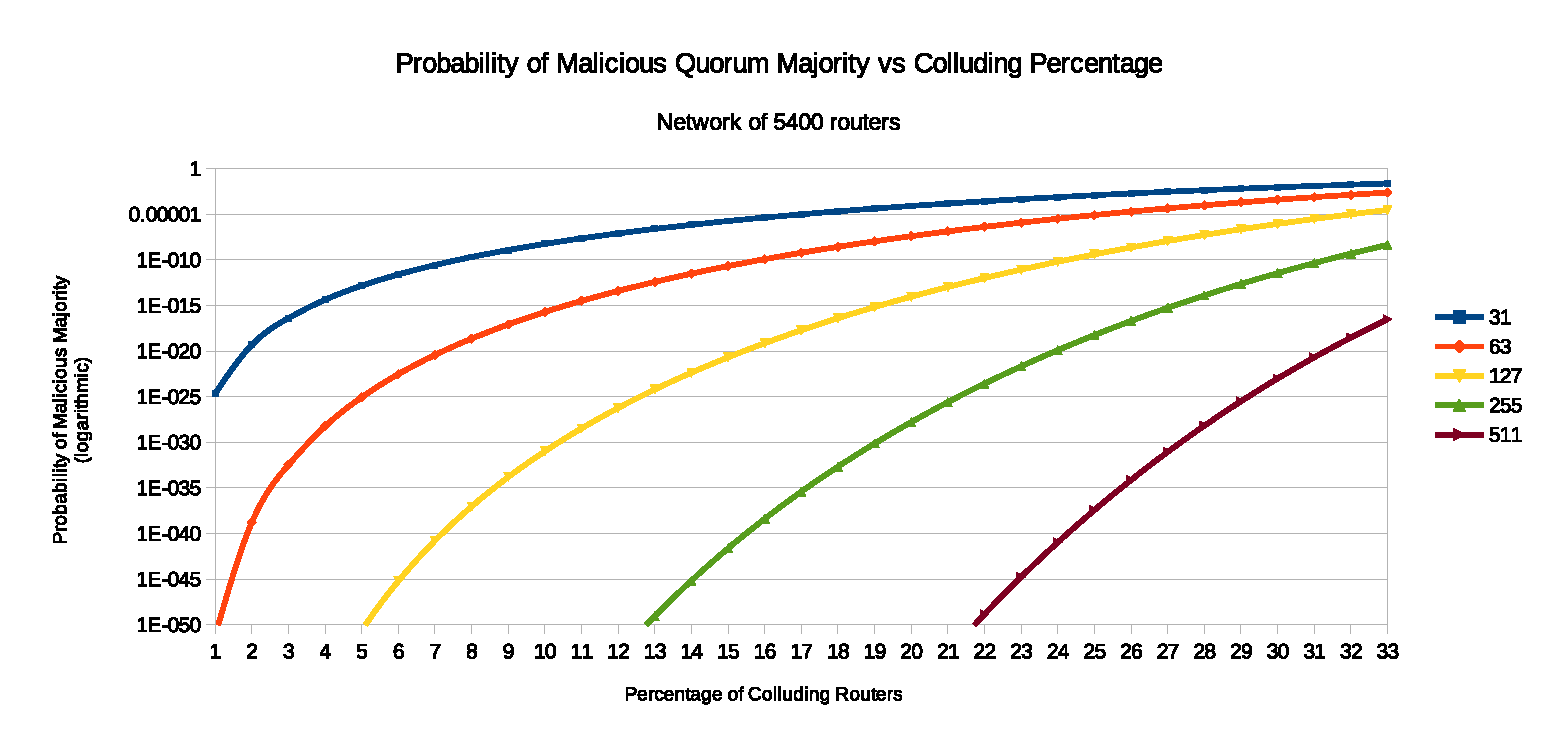
\includegraphics[width=1\textwidth]{analysis/MaliciousQuorumProbability.eps}
	\caption{The probability that Eve controls the majority of the Quorum is given by the PMF of the hypergeometric distribution. We fix $ N $ at 5,400 nodes and graph Eve's success probability as a function of an increasing percentage of Eve-controlled colluding routers. We examine five selections for $ L_{Q} $: 31, 63, 127, 255, and 511. We do not consider percentages beyond 33 percent as 33 percent represents a complete compromise of the Tor network: it is near 100 percent that the three routers selected during circuit construction are under Eve's control, a violation of our security assumptions.}
	\label{chart:quorumMajority}
\end{figure}

Figure \ref{chart:quorumMajority} shows that a choice of $ L_{Q} = 31 $ is suboptimal: the probabilities are above the $ 10^{-38.532} $ threshold for even small levels of collusion. $ L_{Q} = 63 $ likewise fails with approximately two percent collusion, although choices of 127, 255, and 511 fail at levels above approximately 8, 16, and 25 percent, respectively. The figure also suggests that larger Quorums are superior with respect to security. Small Quorums are also less resilient to DDOS attacks at the Quorum in general.

If we assume that Eve controls 10 percent of the Tor network, then we can examine the impact of the longevities of Quorums; over a fixed period of time, slower rotations suggests a lower cumulative chance of selecting any malicious Quorum. If $ w $ is Eve's chance of compromise, then her cumulative chances of compromising any Quorum is given by $ 1 - (1-2)^t $. This gives us a bound estimate on $ \Delta q $. We estimate this over 10 years in Figure \ref{chart:cumulativeProbability}.

\begin{figure}[htbp]
	\centering
	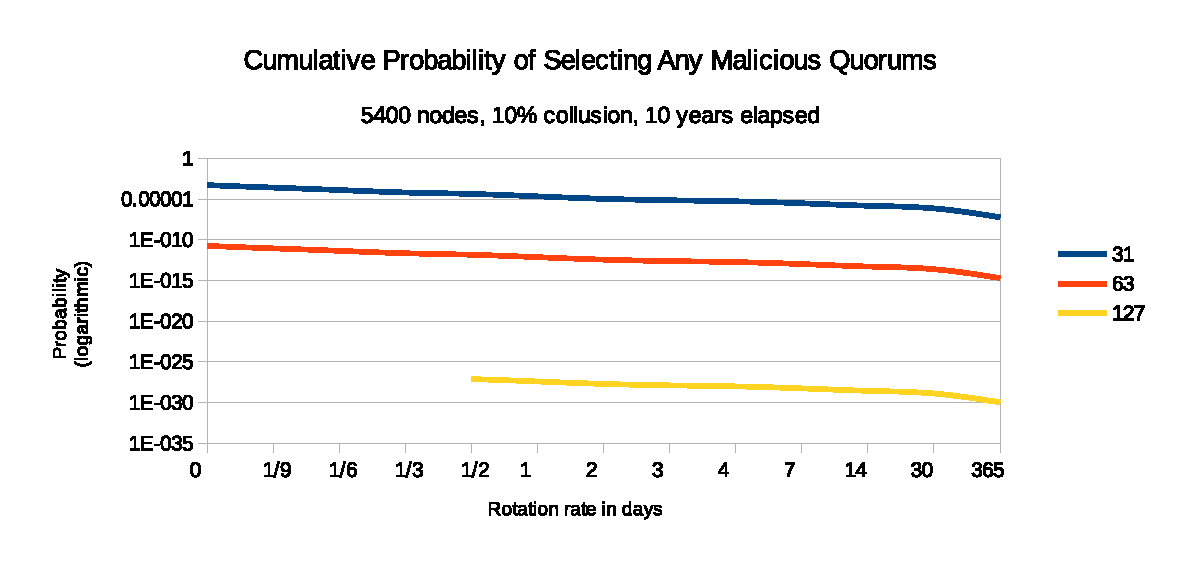
\includegraphics[width=1\textwidth]{analysis/CumulativeMaliciousQuorum.eps}
	\caption{The cumulative probability that Eve controls any Quorum at different rotation rates. We assume 10 percent collusion in a network of 5400 Tor routers, and view across 10 years. We do not graph $ L_{Q} $ values of 255 or 511 as they generate probabilities far below our $ 10^{-38.532} $ threshold; $ L_{Q} = 255 $ and $ L_{Q} = 511 $ produce values less than $ 10^{-58} $ and $ 10^{-134} $, respectively.}
	\label{chart:cumulativeProbability}
\end{figure}

Figure \ref{chart:cumulativeProbability} suggests that while slow rotations (i.e a period of 7 days) generates orders of magnitude less chance than fast rotations, the choice of $ L_{Q} $ is far more significant. Like Figure \ref{chart:quorumMajority}, it also shows that $ L_{Q} = 31 $ and $ L_{Q} = 61 $ are relatively poor choices.

If a selected Quorum is malicious, fast rotation rates will minimize the duration of any disruptions, as shown in Figure \ref{chart:quorumLongevity}. This figure suggests that fast rotations are optimal in that respect, a contradiction to Figure \ref{chart:quorumMajority}. However, given the very low statistical likelihood of selecting a malicious Quorum, we consider this a minor contribution to the decision.

\begin{figure}[htbp]
	\centering
	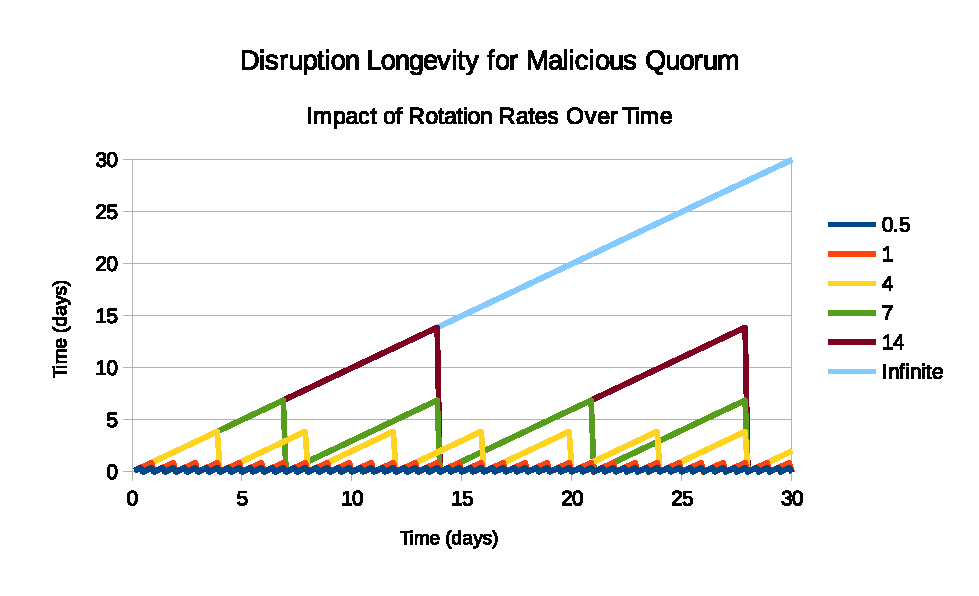
\includegraphics[width=1\textwidth]{analysis/MaliciousLongevityRotations.eps}
	\caption{The duration of malicious Quorums as a function of different rotation rates. Quorums that have very short livetimes (and are thus rotated quickly) minimize the duration of any malicious activity.}
	\label{chart:quorumLongevity}
\end{figure}

Although a malicious Quorum would have the capabilities to deploy a variety of attacks on the network, the proper selections of $ L_{Q} \geq 127 $ and $ \Delta q \geq 1 $ reduces the likelihood of this occurring to near-zero probabilities. We consider this a stronger solution than introducing countermeasures to those attacks. Based on our security analysis, we suggest $ L_{Q} \geq 127 $ and $ \Delta q \geq 1 $.

\newpage

\subsection{Entropy of Tor Consensus Documents}
\label{sec:docEntropy}

We use Tor's consensus documents as a sources of entropy agreed upon by all parties, however we have not yet demonstrated that the network status contains enough entropy to provide reasonable assurance that Eve cannot guess the next Quorum in advance. If Eve could predict future Quorums, Eve can subvert the Quorum Derivation protocol in a variety of attack vectors. However, this would fail our security assumption against adaptive compromise in the presence of OnioNS. Rather than introducing defences against these attack vectors, we nevertheless believe that ensuring sufficient entropy in the consensus documents is a superior defence.

%	\item \textbf{dir-source:} The authority's nickname, fingerprint, IP address, onion routing port, and directory port.
%	\item \textbf{contact:} Optional contact information for the authority operator.
%	\item \textbf{vote-digest:} The hash of the authority's status vote document.
%	
%	\item \textbf{r:} The router's nickname, fingerprint, time of last restart, IP address, onion routing port, and directory port.
%	\item \textbf{m:} The SHA-256 hash of the router's microdescriptor. This also includes its entries in the \emph{cached-microdescs} document (discussed below).
%	\item \textbf{s:} A list of the router's status flags, as given by the directory authorities. Common examples include Running, Valid, Fast, Guard, Stable, and Exit.
%	\item \textbf{v:} The version of the Tor software that the router is running, as reported by the router.
%	\item \textbf{w:} The estimated bandwidth that this router is capable of. This value is determined by speed tests from bandwidth authorities, who are a subset of the directory authorities.

In section \ref{sec:ConsensusDocs} we detailed the significant contents of the three consensus documents relevant to OnioNS, \emph{cached-certs}, \emph{cached-microdesc-consensus}, and \emph{cached-microdescs}. As we stated in section \ref{sec:Protocols}, the Quorum Derivation protocol only utilizes the \emph{cached-certs} and \emph{cached-microdesc-consensus} documents for reasons we discuss below.

\subsubsection{cached-certs}

The \emph{cached-certs} document contains long-term directory identity keys and medium-term signing keys. While Eve cannot predict the public half of new signing keys in advance, the keys rotate every 3-12 months\cite{TorDirSpec} so \emph{cached-certs} is not a timely source of entropy. Nevertheless, if an attacker can predict the network status described in \emph{cached-microdesc-consensus}, the rotation timeline of the signing keys in \emph{cached-certs} places an absolute upper-bound on the duration of Quorum predictability.

\subsubsection{cached-microdesc-consensus}

The \emph{cached-microdesc-consensus} document describes the network status and is our main source of entropy. In the header, the  \emph{vote-digest} header is the hash of a directory authority's status vote. Each directory operates independently and there are nine directory authorities, so we consider this value unpredictable. Router descriptors follow the header in the body of the document. 

The $ r $ field in a router's descriptor contains routing information and time of last restart. Tor routers have no guarantee of availability and routers may restart for a variety of reasons. As of April 2015 Tor's network consists of approximately 7,000 routers \cite{TorMetrics} and assuming that a given router restarts every 60 days, statistically the number of unpredictable $ \emph{r} $ fields each day is given by $ \frac{7000}{60} \approx 116.66 $. Tor displays the restart time down to the second, so each restart adds approximately six bytes of entropy, for an estimated total of $ \frac{7000 * 6}{60} = 700 $ bytes of short-term entropy from the $ r $ field.

%The $ s $ field contains a list of flags given to the router by the directory authorities according to qualification rules. $ s $ is thus predictable if an attacker can monitor the descriptor

The $ v $ field describes the version of Tor that the router is running. Although the versions of Tor are publicly known and the official and unofficial Linux repositories are publicly accessible, Eve cannot predict when an administrator will upgrade their router to the next available Tor version. Although new versions of Tor are not frequently released and routers are upgraded infrequently as shown in Figure \ref{fig:TorVersions}, the $ v $ field still introduces a degree of medium-term entropy into the document.

\begin{figure}[htbp]
	\centering
	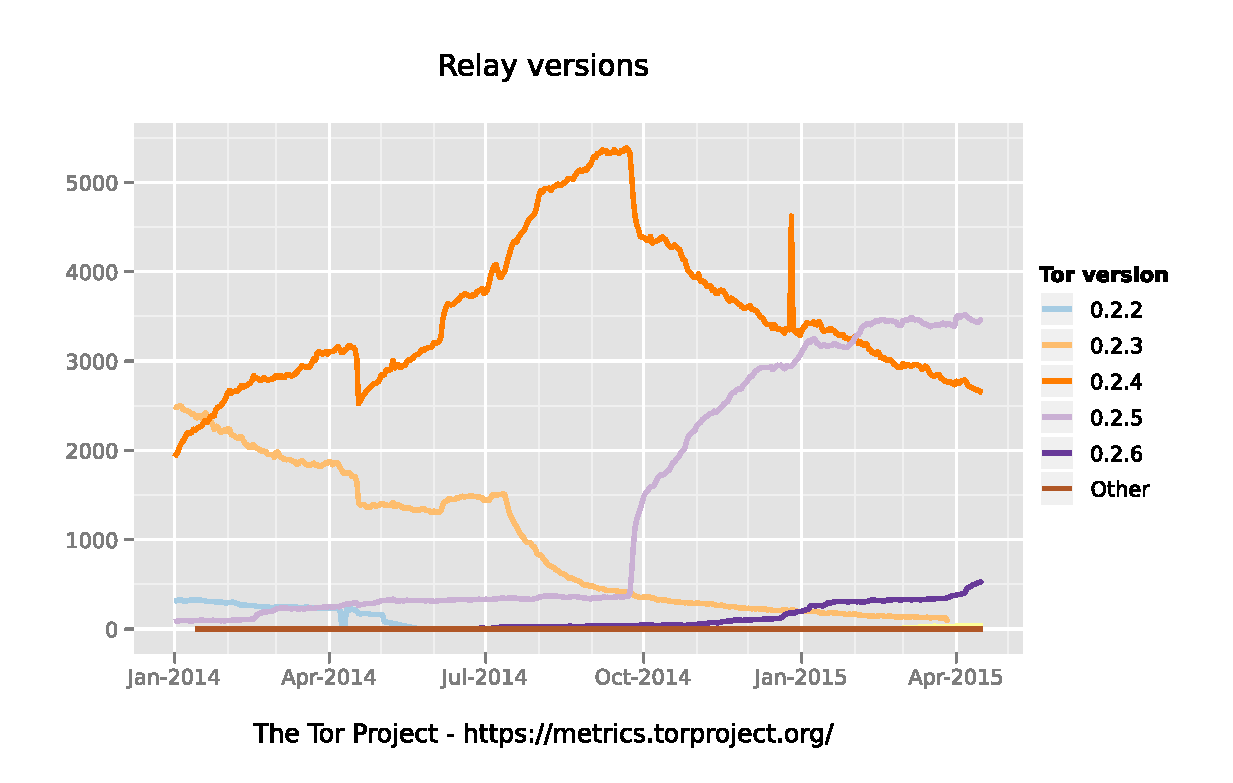
\includegraphics[width=0.95\textwidth]{images/Tor/versions_2014-01_2015-04.eps}
	\caption{The versions of Tor software between January 2014 and April 2015.\cite{TorMetrics}}
	\label{fig:TorVersions}
\end{figure}

The $ w $ field contains the router's estimated bandwidth capacity as calculated by bandwidth authorities. Clients use this field during circuit construction; routers with a higher bandwidth capacity relative to the rest of the network have a higher probability of being included in a circuit. Although it is likely that a given router will have similar bandwidth measurements between consecutive consensus documents, Eve cannot predict the exact performance of a router from the perspective of the bandwidth authority. Eve's capacity to predict the performance of all routers falls outside of Tor's and OnioNS' security assumptions; Eve must therefore be a global attacker who would be capable of compromising the Tor network as a whole anyway.

We note that significant amounts of additional entropy could be trivially added into \emph{cached-microdesc-consensus} if each router added a single random byte to their descriptor or if the directory authorities each contributed entropy.

\subsubsection{cached-microdescs}

Although we did not detail it in section \cite{TorDirSpec}, in practice Tor places client-side timestamps inside \emph{cached-microdescs}. These timestamps would significantly divide the network, causing \emph{cached-microdescs} to be ill-suited for inclusion in the Quorum Derivation protocol. Although \emph{cached-microdescs} contains long-term router keys and the fingerprints of routers in the same family which would both serve as a source of long-term entropy, \emph{cached-microdesc-consensus} contains the SHA-256 hashes of the router descriptor. We therefore do not include it when hashing the documents in the Quorum Derivation protocol.

\subsubsection{General Analysis}

The Quorum Derivation protocol describes initializing the Mersenne Twister with a 384-bit seed. If we assume that Eve desires that the Quorum Derivation protocol produce a Quorum pleasing to Eve (such as including her malicious routers in the Quorum or rejecting specific honest routers from the Quorum) then Eve can find $ k $ seeds that generates a desirable scrambled list in $ 2^{192} $ operations on average, or $ 2^{384} $ operations in the worst case. The chance of any of those seeds being selected is $ \frac{2^{384}}{k} $. 

If we also assume that Eve can predict some fraction $ f \in {(0, 1)} $ of the contents of the consensus documents, then Eve may attempt to manipulate her router's descriptors such that the Quorum Derivation protocol produces one of the $ k $ hashes. SHA-384's strong resistance to preimage and second preimage attacks requires $ 2^{192} $ operations on average for Eve to find one of the $ k $ hashes. This difficulty is compounded by the limited combinatorics within the set of valid router descriptors. The number of operations involved in this attack vector is significantly more than the operations involved in breaking AES, so we disregard the possibility of manipulating the Quorum Derivation protocol in this way. We do not consider the possibility of Eve controlling the entire consensus document, this would severely compromise the integrity of the Tor network and thus violates our security assumptions.

\subsection{Sybil Attacks}

Eve may also attempt to increase her probability of including her malicious nodes in the Quorum via Sybil attacks. We offer no defence against this type of attack, although Tor does. The attack is difficult to carry out in practice due to the slow build of trust within the Tor network. Directory authorities would give Eve's nodes the Fast and Stable flags after weeks of continual uptime and a history of reliability. For large-scale Sybil attacks, this introduces a significant time and financial cost to Eve. We also note that choices of $ L_{Q} $ and $ \Delta q $ also offer significant statistical defences against Sybil attacks, as illustrated in Figures  \ref{chart:quorumMajority} and \ref{chart:cumulativeProbability}, shown above.

\subsection{Hidden Service Spoofing}

OnioNS does not require a hidden service operator to reveal any personally-identifiable information. Hidden services are only known by their public key and domain names, and we assume that the hidden service is authentic. We have also observed spoofed hidden services in the wild, suggesting that this problem already exists in Tor's environment. We do not introduce a reputation system or distributed verification system, and note that it is difficult if not impossible to construct a reliable defence against hidden service spoofing attacks due to their anonymous nature. 

One possible solution, although it severely compromises anonymity, is to register a hidden service with an SSL Certificate Authority and apply an SSL certificate to the server. In this way, TLS communication provides an authenticity check against the hidden service, although TLS also sets up a redundant encryption layer that may decrease performance. However, in practice this solution is very rarely seen; out of approximately 25,000 hidden services,\cite{TorMetrics}\cite{kadianakis2015extrapolating} to date only three hidden services have browser-trusted SSL certificates: Blockchain.info at https://blockchainbdgpzk.onion, Facebook at https://facebookcorewwwi.onion, and The Intercept's SecureDrop instance at https://y6xjgkgwj47us5ca.onion. In future work we may study the security implications of signing the .onion address or the .tor OnioNS domain name. Due to their severe privacy concerns and the security controversy surrounding the centralized CA Chain of Trust, generally speaking we do not recommend the application of SSL certificates to Tor hidden services. 

\subsection{Outsourcing Record Proof-of-Work}

%Scrypt introduces a cost and its memory demands increases the difficulty of custom hardware and massively-parallel attacks, effectively limiting adversaries to the same hardware as legitimate users.

The Record Generation protocol can safely take place within an offline machine under the operator's control. We designed the Record Generation protocol with the objective of requiring the hidden service operator to also perform the scrypt proof-of-work. However, our protocol does not entirely prevent the operator from outsourcing the computation to secondary resource in all cases.

Let Bob be the hidden service operator, and let Craig be a secondary computational resource. We assume that Craig does not have Bob's private key. Then,

\begin{enumerate}
	\item Bob creates an initial Record $ R $ and completes the \emph{type}, \emph{nameList}, \emph{contact}, \emph{timestamp}, and \emph{consensusHash} fields.
	\item Bob sends $ R $ to Craig.
	\item Let $ \mathit{central} $ be $\mathit{type} \concat \mathit{nameList} \concat \mathit{contact} \concat \mathit{timestamp} \concat \mathit{consensusHash} \concat \mathit{nonce} $.
	\item Craig generates a random integer $ K $ and then for each iteration $ j $ from 0 to $ K $,
		\begin{enumerate}
			\item Craig increments \emph{nonce}.
			\item Craig sets \emph{PoW} as $ \mathrm{PoW}(\mathit{central}) $.
			\item Craig saves the new $ R $ as $ C_{j} $.
		\end{enumerate}
	\item Craig sends all $ C_{0 \le j \le K} $ to Bob.
	\item For each Record $ C_{0 \le j \le K} $ Bob computes
		\begin{enumerate}
			\item Bob sets \emph{pubHSKey} to his public RSA key.
			\item Bob sets \emph{recordSig} to $ S_{d}(m, r) $ where $ m = \mathit{central} \concat \mathit{pow} $ and $ r $ is Bob's private RSA key.
			\item Bob has found a valid record if $ H(\mathit{central} \concat \mathit{pow} \concat \mathit{recordSig}) \leq 2^{\mathit{difficulty} * \mathit{count}} $
		\end{enumerate}
\end{enumerate}

% todo: calculate chances of Craig computing a correct record

Our protocol ensures that Craig must always compute more scrypt iterations than necessary; Craig cannot generate \emph{recordSig} and thus cannot compute if the hash is below the threshold. Moreover, the scrypt work incurs a cost onto Craig that must be compensated financially by Bob. Thus the Record Generation protocol places a lower bound on the cost paid by Bob.

%\subsection{False Negatives Claims}
%
%OnionNS records are self-signed and include the hidden service's public key, so anyone --- particularly the client --- can confirm the authenticity (relative to the authenticity of the public key) and integrity of any record. This does not entirely prevent Sybil attacks, but this is a very hard problem to address in a distributed environment without the confirmation from a central authority. However, the proof-of-work component makes record spoofing a costly endeavour, but it is not impossible to a well-resourced attacker with sufficient access to high-end general-purpose hardware.
%
%Hidden service .onion addresses will continue to have an extremely high chance of being securely unique as long the key-space is sufficiently large to avoid hash collisions.
%
%As we have stated earlier, falsely claiming a negative on the existence of a record is a problem overlooked in other domain name systems. One of the primary challenges with this approach is that the space of possible names so vast that attempting to enumerate and digitally sign all names that are not taken is highly impractical. Without a solution, this weakness can degenerate into a denial-of-service attack if the DNS resolver is malicious towards the client. Our counter-measure is the highly compact hashtable bitset with a Merkle tree for collisions. We set the size of the hashtable such that the number of collisions is statistically very small, allowing an efficient lookup in $ \mathcal{O}(1) $ time on average with minimal data transferred to the client.

\subsection{DNS Leakage}

Human mistakes can also compromise user privacy. One such security threat is the accidental leakage of .tor lookups over the Internet DNS. This vulnerability is not limited to OnioNS and applies to any alternative DNS; users may mistakenly attempt lookups over the traditional Internet DNS. Mohaisen and Thomas observed .onion lookups on root DNS servers at a frequency that corresponded to external global events, highlighting the human factor in those leakages.\cite{thomasmeasuring} For OnioNS, this may occur if their client software was not properly configured, if their browser was not properly configured to or could not communicate with Tor, or for other reasons. We offer no defence against this attack vector and note that any defence against it would need to introduce lookup whitelists or blacklists into common browsers such as Chrome, Firefox, and Internet Explorer to prevent them from attempting lookups for pseudo-TLDs.

%\section{Reliability}

%\subsubsection{Flooding}

%\emph{What happens if Quorum nodes are unavailable? How is their unavailability secured for future reference? What are the implications of a Quorum node withholding or forging a Record before flooding their Snapshot out? Can a single node mislead the rest of the Quorum?}

%Although this approach does not entirely thwart Sybil attack, this attack vector is difficulty to impossible to counter in a privacy-enhanced environment, and trading anonymity for defence is highly undesirable.

%\emph{Tor nodes provide no guarantee of availability. What are the implications of Quorum nodes or Mirrors suddenly disappearing? How can data be lost? What if a Quorum node is offline temporarily during active duty, will it catch up?}

%  on Unreliable Hosts

%Tor nodes have no reliability guarantee and may disappear from the network momentarily or permanently at any time. Old \emph{quorums} may disappear from the network without consequence of data loss, as their data is cloned by current \emph{mirrors}. So long as the \emph{quorum} nodes remain up for the $ \Delta i $ days that they are active, the system will suffer no loss of functionality. Nodes that become temporarily unavailable will have out-of-sync \emph{pages} and will have to fetch recent records from other \emph{quorum} nodes in the time of their absence.

\section{Objectives Assessment}

OnioNS achieves all of our original requirements:

\begin{enumerate}
	\item \textbf{The system must support anonymous registrations} --- OnioNS Records do not contain any personal or location information. The PGP key field is optional and may be provided if the hidden service operator wishes to allow others to contact him. However, the operator may be using an email address and a Web of Trust disassociated from his real identity, in which case no identifiable information is exposed.
	\item \textbf{The system must support privacy-enhanced lookups} --- OnioNS performs Domain and Onion Queries through Tor circuits, and under our original assumption that circuits provide strong guarentees of client privacy and anonymity, resolvers cannot sufficiently distinguish users to track their lookups.
	\item \textbf{Clients must be able to authenticate registrations} --- OnioNS Records are self-signed, enabling Tor clients to verify the digital signature on the domain names and check the public key against the server's key during the hidden service protocol. This ensures that the association has not been modified in transit and that the domain name is authentic relative to the authenticity of the destination server.
	\item \textbf{Domain names must be provably or have a near-certain chance of being unique} --- Tor hidden services .onion addresses are cryptographically generated with a key-space of $ 58 ^ {16} \approx 2 ^ {93.727695922} $ and domain names within OnioNS are provably unique by anyone holding a complete copy of the Pagechain.
	\item \textbf{The system must be distributed} --- The responsibilities of OnioNS are spread out across many nodes in the Tor network, decreasing the load and attack potential for any single node. The Pagechain is likewise distributed and locally-checked by all Mirrors, and although its head is managed by the Quorum, these authoritative nodes have temporary lifetimes and are randomly selected. Moreover, Quorum nodes do not answer queries, so they have limited power.
	\item \textbf{The system must be simple and relatively easy to use} --- Domain Queries are automatically resolved and require no input by the user. From the user's perspective, they are taken directly from a meaningful domain name to a hidden service. Users no longer have to use unwieldy .onion addresses or review third-party directories, OnioNS introduces memorability to hidden service domains.
	\item \textbf{The system must be backwards compatible with existing protocols} --- OnioNS does not require any changes to the hidden service protocol and existing .onion addresses remain fully functional. Our only significant change to Tor's infrastructure is the mechanism for distributing hashes for the Quorum Qualification protocol, but our initial technique for using the Contact field minimizes any impact. We also hook into Tor's TLD checks, but this change is very minor. Our reference implementation is provided as a software package separate from Tor per the Unix convention.
\end{enumerate}

Finally, we meet our optional performance objectives:

\begin{enumerate}
	\item \textbf{The system should not require clients to download the entire database} --- Only Mirrors hold the Pagechain, and clients do not need to obtain it themselves to issue a Domain Query. Therefore clients rely on their existing and well-established trust of Tor routers when resolving domain names. However, clients may optionally obtain the Pagechain and post Domain Queries to localhost for greater privacy and security guarantees.
	\item \textbf{The system should not introduce significant burdens to the clients} --- Record verification should occur in sub-second constant time in most environments, and Ed25519 achieves very fast signature confirmation so verifying Page signatures at level 1+ takes trivial time. However, clients also verify the Record's proof-of-work, so for some scrypt parameters the client may spend non-trivial CPU time and RAM usage confirming the one scrypt iteration required to check. We must therefore choose our parameters carefully to reduce this burden especially on low-end hardware.
	\item \textbf{The system should have low latency} --- Domain Queries without any packet delays over Tor low-latency circuits. Its exact performance is largely dependent on circuit speed and the client's verification speed.
\end{enumerate}

We therefore believe that we have squared Zooko's Triangle; OnioNS is distributed, enables hidden service operators to select human-meaningful domain names, and domain names are guaranteed unique by all participants.

	
\chapter{\uppercase{Results}}

\section{Implementation}

implementation...

\section{Discussion}

discussions...

\subsection{Guarantees}

Guarantees...
	%
\chapter{FUTURE WORK}

We introduce no changes to Tor's hidden service protocol and also note that the existence of a DNS system introduces forward-compatibility: developers can replace hash functions and PKI in the hidden service protocol without disrupting its users, so long as records are transferred and OnionNS is updated to support the new public keys.

web of trust for .onion keys to thwart Sybil attack

Some open problems that I need to address include:

\begin{enumerate}
	\item How frequently should domains expire? Are there any security risk in sending a Renew request?
	\item How should unreachable or temporarily down nodes be handled? I'd like to know the percentage of the Tor network that is reachable at any given time.
	\item How many nodes in the Tor network should be assumed to be actively malicious? What are the implications of increasing this percentage?
	\item What attack vectors are there from the committee nodes, and how can I thwart the attacks?
	\item What are the implications of a node intentionally voting the opposite way, or ignoring the request altogether?
	\item What would happen if a node was too slow or did not have enough storage space to do its job properly?
	\item What other open problems are there?
	\item What related works are there in the literature that relate to the concepts I have created here?
\end{enumerate}
	
\chapter{CONCLUSION}

OnionNS is a distributed DNS system inside the Tor network. The system maps human-meaningful .tor domain names to traditional Tor .onion addresses. It exists on top of current Tor hidden service infrastructure and increases usability of hidden services by abstracting away the base58-encoded hidden service addresses. OnionNS is powered by a randomly chosen set of Tor nodes, whose work can be verified by any party with a copy of Tor's consensus document. Records are self-signed and can be publicly verified. If accepted by the Tor community, OnionNS will be a valuable abstraction layr that will significantly improve the usability and popularity of Tor hidden services.


	\references{thesis}{IEEEtran.bst}

	%\include{appendix} % optional
	%\include{vita}     % optional
	%}}}
\end{document}
